\vspace{10pt}

\minitoc
\clearpage

% % % % % % % % % % % % % % % % % % % % % % % % % % % % % % % % % % %
% Odométrie visuelle et reconstruction de l'environnement statique  %
% % % % % % % % % % % % % % % % % % % % % % % % % % % % % % % % % % %

\section{Introduction}
% On fait le constat que les informations obtenues précédemment ne sont pas suffisantes
Suite à l'étape précédente de perception visuelle par un dispositif de stéréo-vision, on dispose à cet étape d'un ensemble de points repérés dans le plan image et suivis dans le temps. On peut également le représenter comme une séquence de nuages de points positionnés en trois dimensions, et dont les associations temporelles individuelles sont connues. Ces informations ne sont pas de nature à répondre à certains de nos besoins, identifiés dans la section \ref{sec:ch1_besoins}, par exemple le positionnement du porteur dans son environnement ou la détection de l'espace navigable. Elles ne sont, par ailleurs, pas de qualité suffisante pour répondre précisément à d'autres tâches qui nous sont imputées, par exemple la détection des obstacles statiques, du fait d'un bruit de mesure très important.\\
% Conséquence : intégrer ces informations dans le temps -> on a besoin de déterminer l'ego-motion et de proposer un cadre pour la fusion des observations
Il est alors naturel de s'intéresser à l'intégration temporelle de ces mesures, afin d'améliorer leur précision par l'accumulation des observations, et d'obtenir les informations qui nous font défaut. Deux besoins sont immédiatement perceptibles : le mouvement du porteur doit être déterminé, afin de rendre ces observations cohérentes ; et une fusion de ces observations permettant d'obtenir des valeurs estimées doit être proposée. Ces deux problématiques sont intrinsèquement liées\footnote{Une erreur sur l'estimation du mouvement a en effet une incidence directe sur la qualité de l'accumulation des observations, tandis que ces observations sont elles-mêmes à la source de cette estimation.}, ce que leur estimation prend souvent en compte. On notera dans la suite \emph{ego-motion} le mouvement propre du porteur, comme il  est l'usage dans la littérature.\\
% Rapport au SLAM et résolution disjointe mouvement/position des points
Plusieurs méthodes présentes dans l'état de l'art proposent une résolution simultanée de ces deux problématiques, comme nous l'avons évoqué dans la section \ref{sec:ch2_Algo_total}, ce qui semble naturel du fait de leurs interactions. Cette approche est cependant intrinsèquement limitée dans le nombre de points qui peut alors être positionné, du fait de l'augmentation très rapide des dimensions du problème. Nous avons fait le choix d'une résolution disjointe, afin de pouvoir augmenter très nettement la densité de points traités par rapport à ces techniques, tout en conservant un temps de calcul raisonnable.\\
% Présentation du plan
On présentera quelques uns de ces enjeux dans une première partie, avec une revue de l'état de l'art dans les domaines de l'odométrie visuelle, et de la construction de nuages de points à partir d'observations multiples. On détaillera également quelques techniques parmi les plus utilisées en matière de filtrage et d'estimation robuste, ces techniques étant exploitées dans notre proposition. Une seconde partie nous permettra de présenter l'algorithme que nous proposons, pour estimer l'\emph{ego-motion} et la position des points observés, dont le fonctionnement général est décrit sur la figure \ref{fig:ch4_schéma_global}. Une troisième et dernière partie nous permettra d'aborder l'implémentation de notre proposition, ainsi que son évaluation sur des critères de précision ou de temps de calcul.

\begin{figure}
	\centering
	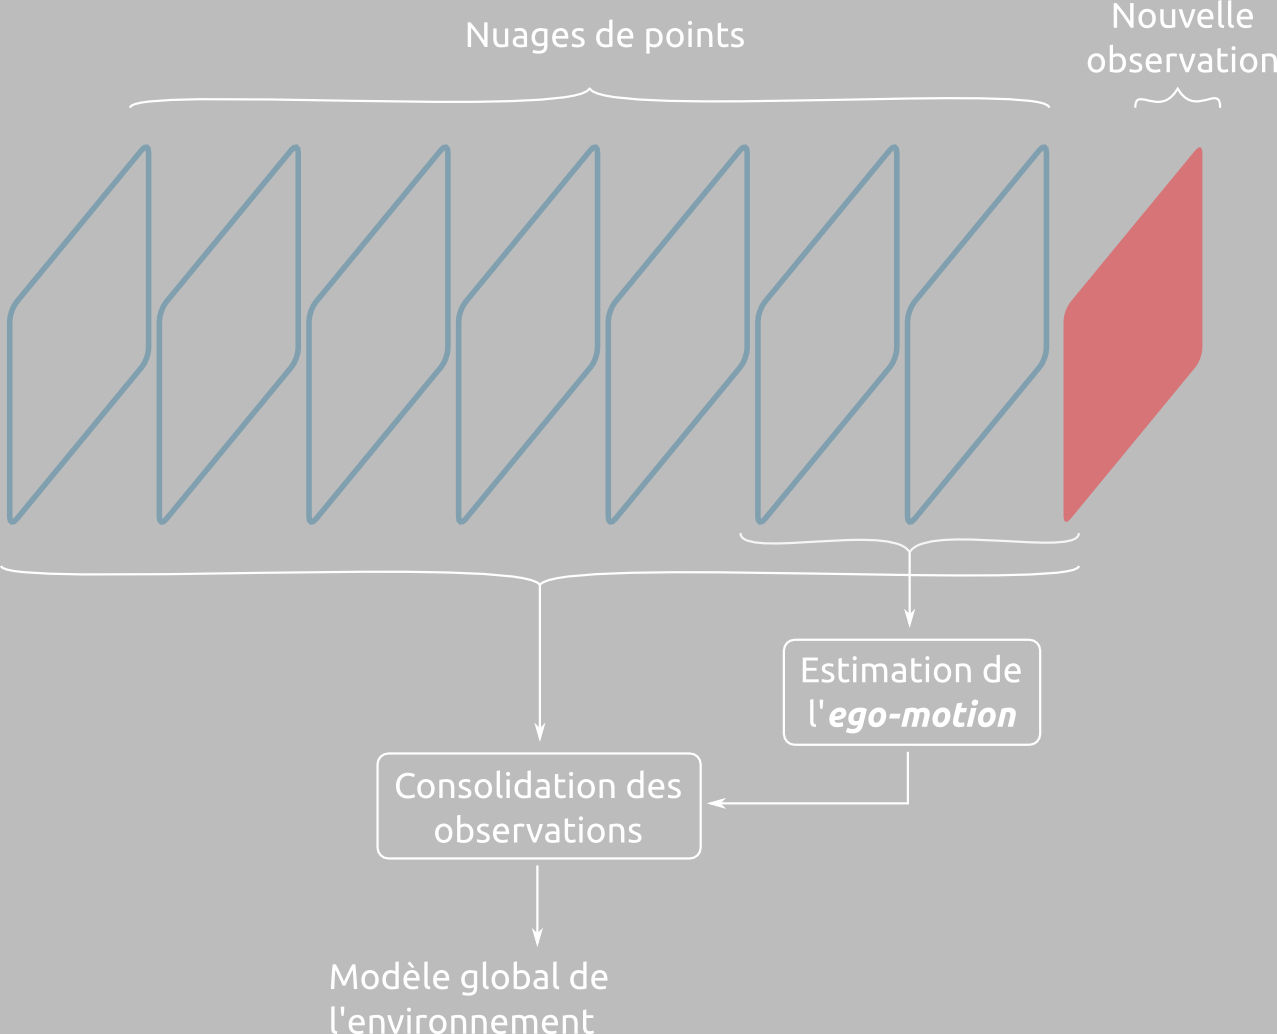
\includegraphics[width=0.8\textwidth]{Chapter4/graphics/overall_scheme.png}
	\caption{Représentation schématique du procédé proposé pour consolider les observations dans le temps et dans le référentiel du porteur. Les observations précédentes sont supposées  être dans un référentiel cohérent, la nouvelle observation étant associée à un nouveau référentiel.}
	\label{fig:ch4_schéma_global}
\end{figure}

\section{État de l'art} \label{sec:ch4_state_of_art}
On présente dans ce qui suit un état de l'art des méthodes répondant à tout ou partie de nos besoins. Il s'agit ainsi de recenser les techniques les plus efficaces en matière d'odométrie visuelle et de reconstruction de l'environnement à partir d'observations multiples, tout en conservant nos prérequis initiaux d'une exécution en temps réel et sur un grand nombre de points. On présente également quelques éléments de compréhension dans des domaines spécifiques, celui des estimateurs robustes et du filtrage, ces domaines étant mis à contribution dans l'approche  que nous proposons pour déterminer le mouvement du porteur.

\subsection{Odométrie visuelle} \label{sec:ch4_state_of_art_VO}
On distingue dans la suite les méthodes se situant dans l'espace image et les méthodes considérant l'espace en trois dimensions pour estimer l'ego-motion. Ces techniques peuvent être plus précisément classées selon l'espace dans lequel est reportée l'erreur d'estimation, c'est à dire l'erreur que l'on cherche à minimiser pour estimer le mouvement du porteur entre deux acquisitions. Ceci n'exclue pas nécessairement que l'une ou l'autre des représentations soit mise à contribution en tant qu'intermédiaire de calcul. On considère par ailleurs l'ensemble des techniques d'odométrie visuelle, qu'elles soient basées sur une configuration de type mono-vision ou stéréo-vision. \\
Il est souvent préférable de se situer pour cette estimation dans l'espace du capteur, c'est à dire dans le plan image dans notre cas. Changer de système de coordonnées (par exemple pour repasser dans l'espace en trois dimensions) peut en effet impliquer de faire intervenir des fonctions non-linéaires complexes, qui modifient notamment la forme de l'incertitude sur la mesure. Les traitements ultérieurs envisagés dans un système global de perception, en amont ou en aval de cette étape d'odométrie visuelle, peuvent cependant rendre une estimation dans l'espace 3D pertinente.
% Revenir sur la nécessité d'un suivi dans le temps -> suivi de point, de structure, d'une autre caractéristique (foyer d'expansion ?)

\subsubsection{Méthodes mono-caméra}
\paragraph{Approches classiques:\\}
% Première méthodes basées sur le déplacement d'éléments particuliers
L'estimation du mouvement à partir d'une séquence d'images est un problème ancien mais toujours étudié, et de nombreuses propositions sont présentes dans la littérature pour tenter d'y répondre. Notre synthèse de ce domaine ne sera sans doute pas exhaustive, mais on tentera d'en présenter les principales caractéristiques, ainsi que leur évolution historique. Les premières méthodes proposées se concentrent sur l'évolution de primitives dans l'image (lignes ou points dont l'identification est aisée), du fait des contraintes en termes de puissance de calcul alors prédominantes. L'utilisation de points plus flexibles (points saillants quelconques), ou du flux optique dans son intégralité est ensuite rapidement proposée. Plusieurs méthodes très diversifiées sont ainsi présentées par Tian \textit{et al} dans (\cite{Tian1996}).\\

La position du foyer d'expansion (point de convergence du flux optique) sert initialement de critère pour la détermination du mouvement rigide de translation entre deux images. Dans le cas d'un mouvement complet (translation et rotation), ces techniques déterminent tout d'abord le foyer d'expansion et la translation, avant de rechercher la composante de rotation du mouvement par minimisation du résidu entre flux optique calculé et observé. Ces considérations sont par ailleurs valables sur une surface planaire, le flux optique devant donc être initialement décomposé. La résistance au bruit de ces techniques repose enfin souvent sur un système de vote (\cite{Adiv1985}), qui privilégie le mouvement faisant consensus au détriment d'erreurs probables si de nombreux objets en mouvement sont observés. Cette dernière approche est toujours utilisée dans une technique plus récente basée sur les tenseurs d'orientation, pour le calcul du flux optique uniquement, la segmentation étant alors établie par croissance de région (\cite{Farneback2000}).\\

\paragraph{Approches globales:\\}
Des méthodes ont par ailleurs un statut particulier dans le domaine de l'odométrie visuelle, car elles résolvent ce problème conjointement avec la construction d'une carte de l'environnement. Il s'agit des approches de type SLAM, qui ont déjà été abordées dans la section \ref{sec:ch2_Algo_total} dans leur variante prenant en compte les objets mobiles de la scène. Deux approches principales sont présentes dans la littérature pour procéder à un SLAM, chacune disposant de points forts spécifiques : par optimisation, ou par filtrage.\\
Une approche par optimisation fonctionne, en général, en recherchant de manière itérative le déplacement minimisant une erreur de re-projection dans le plan image, à partir de points suivis dans le temps. Il s'agit par exemple du procédé proposé par Klein et Murray (\cite{Klein2007}, ou Zou dans une approche combinant si besoin plusieurs caméras (\cite{Zou}). Nister  (\cite{Nister2006}) propose cependant une méthode exploitant une optimisation robuste dans l'espace en trois dimensions. Les techniques suivies pour l'optimisation sont très différentes selon les propositions, une revue succincte pouvant notamment être lue dans \cite{Madsen2004}.\\

Plutôt qu'une estimation par optimisation, une approche par filtrage, souvent basée sur un filtre de Kalman étendu (EKF, \emph{Extended Kalman Filter}), est également possible. Les éléments du filtre sont alors des points singuliers de l'image, dont la position est initialement inconnue. Cette méthode permet notamment la prise en compte élégante d'un modèle de mouvement, qu'il est délicat d'inclure dans les méthodes par optimisation. Le filtrage autorise par ailleurs naturellement la prise en compte de l'historique des observations, dans l'hypothèse où le système est une chaîne de Markov de rang 1. Le nombre de points exploité pour l'estimation du mouvement est en revanche limité par les enjeux du traitement en temps réel. Le filtre de Kalman et ses dérivés nécessitent en effet l'inversion d'une matrice dont la taille est liée au nombres d'éléments du vecteur d'état, lequel croît avec le nombre de points pris en compte (cf. section \ref{sec:ch4_filtrage}). Cette inversion a un coût calculatoire de l'ordre de $O(d^{2.4})$ pour une matrice de dimension $d$, ce qui limite en pratique le nombre de points positionnés à quelques centaines d'unités. Cette méthode a été initialement proposée par Davison (\cite{Davison2003}), et a grandement été perfectionnée par la suite, notamment au niveau de l'initialisation de la covariance des points positionnés (\cite{Eade, Montiel, Ortega2007, Feraud2011}). La sélection des points utilisés doit alors faire l'objet d'une procédure robuste, par exemple grâce à un RANSAC (\emph{Random Sample Consensus}, Consensus à partir d'échantillons aléatoires, Fischler et Bolles \cite{Fischler1981}), pour éviter les erreurs liées au suivi de points mobiles. L'espace dans lequel se situe l'estimation du filtre dépend du modèle de mesure utilisé, mais il s'agit le plus souvent dans la littérature de l'espace image.\\

\subsubsection{Méthodes multi-caméras}
% Positions relative des caméras connue, ou non ?
D'autres techniques que celles présentées précédemment sont rendues possibles par l'utilisation de caméras supplémentaires, dont la configuration est connue ou non. La présence de ces points de vue disjoints permet de limiter les configurations mettant en défaut l'estimation du mouvement, bien que certains cas pathologiques soient toujours possibles (par exemple visible sur la figure \ref{fig:ch4_egomotion_vision_problem}).

\paragraph{Configuration des caméras inconnue:\\}
Ce cas de figure n'est pas courant dans le domaine de la stéréo-vision, mais il peut présenter un intérêt industriel ou expérimental, de part l'usage de caméras non-calibrées. Si la configuration relative des caméras est fixe, il est possible d'exploiter une détermination autonome du mouvement sur chacune des caméras, et d'estimer alors les paramètres de calibration de par les termes croisés induits par l'observation simultanée des mêmes éléments de la scène. Marquez-Gomez et Devy (\cite{Devy}) proposent ainsi d'utiliser un EKF  réparti sur deux caméras (BiCamSLAM) à même de répondre à cette problématique. Tout en conservant le formalisme de l'EKF dans un contexte de SLAM visuel, Bresson \textit{et al.} (\cite{Bresson2012}) proposent un algorithme décentralisé à même de positionner plusieurs entités indépendantes disposant chacune d'une unique caméra. \\
Il est par ailleurs toujours possible de confier à une optimisation globale la résolution des inconnues du système, parmi lesquelles les positions relatives des caméras présentes. Ces positions relatives peuvent alors varier dans le temps, au prix d'un coût calculatoire et d'une perte de précision importantes. Un positionnement collaboratif est alors possible, à partir de caméras individuelles \cite{Zou}, ou de paires de caméras calibrées \cite{Gil2010}.

\paragraph{Configuration des caméras connue au préalable:\\}
% - soit on minimise en 3D, soit on minimise l'erreur dans l'espace du capteur
La connaissance du changement de repère entre les plans image des différentes caméras permet d'obtenir une estimation directe de la position dans l'espace de points visibles simultanément sur chacun de ces plans. Deux approches sont alors possibles pour obtenir une estimation du mouvement, qui peuvent être dissociées par l'espace dans lequel l'erreur résiduelle se situe.\\
\begin{itemize}
	\item{} Dans le premier cas, il s'agit de minimiser par une technique robuste l'erreur dans l'espace en trois dimensions entre plusieurs observations de mêmes éléments, en déterminant ainsi la transformation rigide optimale. Ceci peut être réalisé selon des méthodes d'algèbre linéaire, comme c'est le cas avec d'autres capteurs (on peut ainsi se rapprocher de l'ICP (\emph{Iterative Closest Point}, itérations selon le point le plus proche), algorithme notamment utilisé pour le recalage de nuages de points obtenus par un télémètre laser, qui résout le problème de l'association des points dans le temps par une estimation itérative associant les points les plus proches, voir par exemple \cite{Rusinkiewicz}). Ces méthodes ont fait l'objet de nombreuses publications, et s'inscrivent plus généralement dans l'optimisation par moindres carrés (on pourra notamment voir \cite{Arun1987,Umeyama1991, Goryn1995, Eggert1997}). Une des méthodes de résolution, qui sera présentée dans la section \ref{sec:ch4_svd_pondérée}, exploite l'algèbre linéaire et la décomposition en éléments propres (SVD, \emph{Singular Value Decomposition}) d'une matrice de corrélation. Situant toujours l'erreur que l'on cherche à minimiser dans l'espace en trois dimensions, d'autres techniques permettent de prendre en compte plusieurs acquisitions consécutives dans une optimisation globale. Ces méthodes sont connues sous le nom de "Bundle Adjustment" (Ajustement de rayons), et de nombreux algorithmes sont utilisés dans ce cadre (\cite{Triggs2000}). Leur usage n'était historiquement pas temps réel, mais les progrès conjoints des algorithmes d'optimisation et des processeurs en font maintenant des solutions sérieuses pour l'estimation du mouvement (\cite{Niko2006, Konolige2008}). Une autre technique d'optimisation sur plusieurs observations consécutives est par ailleurs proposée par Lategahn et al. (\cite{Lategahna}), sans cependant prendre en compte (contrairement aux procédures de \emph{Bundle Adjustment}) la position des points observés dans l'espace. \\
	
	\item{} Ces méthodes situant l'optimisation dans l'espace cartésien en 3 dimensions décrivant le repère \og monde\fg{} ne sont en général pas optimales, dans le cas de l'utilisation d'un dispositif de stéréo-vision, comme nous l'avons notamment noté dans \ref{sec:ch2_Modèle Stéréovision} (une étude des conséquences de ce bruit anisotrope est notamment présente dans \cite{Blostein1987} et \cite{Sibley2007}, ce dernier considérant de plus les problèmes de biais liés à une mauvaise calibration). Il est donc souvent intéressant de minimiser une erreur dans le plan image. Celle-ci peut être dérivée explicitement à partir des équations de la stéréo-vision, tout en gardant un caractère linéaire (\cite{Demirdjian2001,Bak2011}). Cette optimisation peut également passer par une résolution non-linéaire à base de descente de gradient (méthodes de Levenberg-Marquardt ou Newton-Raphson), comme proposé dans de nombreuses publications ( \cite{Nister2006, Comport2010, Mei, Comport2010, Zou}). Dans une approche un peu différente, Agrawal\textit{ et al.} (\cite{Agrawal2007}) proposent d'associer l'estimation du mouvement à une fonction de coût robuste basée sur un algorithme de type RANSAC, dans le plan image. Le calcul des hypothèses de mouvement est linéaire et dans l'espace en trois dimensions, à partir des correspondances sélectionnées aléatoirement. Le score qui leur est associé est établi dans l'espace image et l'optimisation est dans ce cas non-linéaire (RANSAC).\\
\end{itemize}

\paragraph{Remarques sur une résolution linéaire adaptée à la stéréovision:\\} \label{ch4:méthode_bak}
Il est possible d'utiliser une méthode matricielle tout en prenant en compte les particularités du bruit de stéréo-vision. Une approche proposée par Bak (\cite{Bak2011}) autorise en effet une résolution élégante de cette problématique. A partir de l'expression des coordonnées des points dans le repère image d'un dispositif de deux caméras (en considérant donc les variables de position sur l'un des plans image, ainsi que la disparité), Bak en dérive l'effet d'une transformation rigide dans l'espace. Il réécrit alors l'équation \ref{eq:ch4_eq_to_minimize} dans le plan image, et obtient une équation linéaire pour laquelle beaucoup d'outils de résolution sont disponibles. Une méthode d'optimisation non-linéaire à base de RANSAC est par ailleurs utilisée pour rendre cette estimation plus robuste. \\
En reprenant les notations de Bak, les coordonnées des points dans l'espace image étendu s'écrivent :

\begin{equation}
	m_i = \left(  
		\begin{array}{c} 
			{x_m}_i		 \\ 
			 {y_m}_i	 \\ 
			{\delta_m}_i
		\end{array}
		\right) 
\end{equation}

Le problème à résoudre, reliant une transformation rigide $(R, T)$ dans l'espace 3D aux coordonnées projetées dans le système de stéréo-vision, s'écrit alors (avec $f$ la focale optique et $b_s$ la distance entre les deux caméras) :

\begin{align}
	\begin{split}
		&\left(
			\begin{array}{cccccc}
				-\frac{{x_m'}_1 \cdot {y_m}_1}{f} 		& -\frac{{x_m}_1 \cdot {x_m'}_1}{f} +f 	& -{y_m}_1 	& \frac{{\delta_m}_1}{b_s} & 0 & \frac{{\delta_m}_1 \cdot {x_m'}_1}{b_s}\\ 
				f -\frac{{y_m}_1 \cdot {y_m'}_1}{f} 	& \frac{{x_m}_1 \cdot {y_m'}_1}{f} 		& -{x_m}_1 	& 0 & \frac{{\delta_m}_1}{b_s} & \frac{{\delta_m}_1 \cdot {y_m'}_1}{b_s}\\ 
				\frac{{\delta'_m}_1 \cdot {y_m}_1}{f} 	& -\frac{{\delta_m'}_1 \cdot {x_m}_1}{f} & 0 & 0 & 0 & \frac{{\delta_m}_1 \cdot {\delta_m'}_1}{b_s}\\ 
				\cdots 									& \cdots 								& \cdots 	& \cdots 	& \cdots 	& \cdots\\ 
				-\frac{{x_m'}_N \cdot {y_m}_N}{f} 		& -\frac{{x_m}_N \cdot {x_m'}_N}{f} +f 	& -{y_m}_N 	& \frac{{\delta_m}_N}{b_s} & 0 & \frac{{\delta_m}_N \cdot {x_m'}_N}{b_s}\\ 
				f -\frac{{y_m}_N \cdot {y_m'}_N}{f} 	& \frac{{x_m}_N \cdot {y_m'}_N}{f} 		& -{x_m}_N 	& 0 & \frac{{\delta_m}_N}{b_s} & \frac{{\delta_m}_N \cdot {y_m'}_N}{b_s}\\ 
				\frac{{\delta'_m}_N \cdot {y_m}_N}{f} 	& -\frac{{\delta_m'}_N \cdot {x_m}_N}{f} & 0 & 0 & 0 & \frac{{\delta_m}_N \cdot {\delta_m'}_N}{b_s}
			\end{array} 
		\right) 
		\cdot  \lvert {
		\begin{array}{c}
			R\\ 
	 		T
		\end{array}
		} \\
		& \hspace*{5cm} = \left( {
		\begin{array}{c}
			{x_m}_1-{x_m'}_1			\\
			{y_m}_1-{y_m'}_1			\\
			{\delta_m}_1-{\delta_m'}_1	\\
			\cdots 						\\
			{x_m}_N-{x_m'}_N			\\
			{y_m}_N-{y_m'}_N			\\
			{\delta_m}_N-{\delta_m'}_N
		\end{array} }
		\right)
	\end{split}
\end{align}

Cette méthode est sans doute plus optimale que celle que nous proposons (section \ref{sec:ch4_robust_estimation}), mais ne profite pas de l'une des caractéristiques de la méthode par décomposition en éléments propres, à savoir sa dépendance très faible au nombre de points pris en compte. Le système à résoudre dans le cas d'une approche dite \og SVD\fg{} est de taille 3x3, quel que soit le nuage de points, tandis que cette approche conduit à un système dont la complexité est de l'ordre de $O(N^2)$. Les temps de calcul attendus sont donc relativement importants, ce que nous souhaitons éviter, au prix d'une perte de précision probable.

\subsubsection{Exploitation de capteurs tiers pour l'estimation de l'\textit{ego-motion}}
L'estimation de l'ego-motion à partir des informations visuelles peut ne pas être suffisante pour satisfaire tous les prérequis d'une navigation autonome. La vision peut ainsi être intrinsèquement mise en défaut (illumination problématique, vibrations, etc), tandis que la scène elle-même peut rendre l'odométrie impossible, sans que l'acquisition visuelle soit en faute (mouvement d'un élément tiers emplissant le champ visuel, voir la figure \ref{fig:ch4_egomotion_vision_problem} par exemple). Loin d'être des cas particuliers, ces phénomènes peuvent être couramment rencontrés dans des situations visées par un véhicule autonome au sein d'un cadre de vie propre aux humains, par exemple au sein d'une foule. \\

\begin{figure}
	\centering
	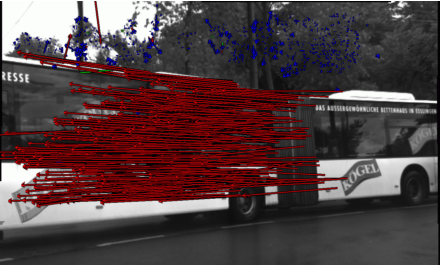
\includegraphics{Chapter4/graphics/problematic_scene.png}
	\caption{Exemple de situation problématique pour l'estimation purement visuelle de l'ego-motion. Les éléments statiques de la scène sont très minoritaires, du fait du masquage produit par un objet mobile. Illustration tirée de l'article \cite{Badino2008}}	
	\label{fig:ch4_egomotion_vision_problem}
\end{figure}

Il est donc assez naturel de chercher à corriger ce problème par la fusion d'informations de plusieurs capteurs complémentaires, comme un odomètre, un outil de positionnement satellitaire global (dit \emph{GNSS, Global Navigation Satellite System} dans la littérature anglo-saxonne, tel que le GPS, GLONASS ou Galiléo), ou encore un capteur de mouvent type IMU. L'utilisation d'un filtre de type EKF ou UKF fournit un cadre élégant pour la fusion de données, les différents capteurs étant associés à un modèle permettant la comparaison de leurs apports sur une base commune. Ce dispositif est particulièrement adapté au traitement temps réel, de part son caractère itératif, et la relative constance du temps de mise à jour. Leur couplage avec un algorithme de détermination de l’\emph{ego-motion} par indices visuels est présent dans la littérature (par exemple \cite{Singh2005,Bak2011}), mais l'utilisation d'autres capteurs est également possible, notamment les télémètres lasers (\cite{Weyers2011}). Une prise en compte par optimisation étant également possible (voir par exemple \cite{Martinelli2012}), même si sa mise en œuvre en temps réel est plus complexe.

\subsection{Génération de l'environnement à partir d'observations successives}
\paragraph{Approches récursives:\\}
La construction d'un nuage de points représentatif de la scène rentre explicitement dans les pré-requis du SLAM, on citera donc ici quelques exemples remarquables de la littérature à ce sujet. Ce sujet a déjà été abordé au point \ref{sec:ch4_state_of_art_VO}, et on pourra donc rapidement aborder la proposition initiale de Davison basée sur un filtre EKF (\cite{Davison2003}), et quelque unes des nombreuses évolutions ont été proposées. Montiel \textit{et al.} (\cite{Montiel}) ont ainsi proposé une paramétrisation améliorée de l'incertitude sur la position des amers visuels lors de leur introduction dans le filtre, afin de mieux gérer la non-linéarité dans l'estimation de la position liée à la distance au capteur (\emph{Inverse Depth Parametrization}). La covariance sur la position de l'amer est liée à l'inverse de sa distance au centre optique, cette paramétrisation étant modifiée pour revenir à une estimation directe dès que l'amer est suffisamment bien localisé). Tout en conservant une estimation par un filtre, Eade et Drummond (\cite{Eade}) proposent un algorithme autorisant la perception d'une carte de dimension beaucoup plus importante : dans la proposition de Davison, le filtre conserve à tout moment les covariances de chacun des amers estimés dans une unique matrice, ce qui rend le processus de mise à jour de l'ordre de O($N^2$) avec $N$ le nombre de points\footnote{Ce coût optimal était jusqu'à 2010 de très exactement $N^{2.376}$ pour l'algorithme de Coppersmith-Winograd (\cite{Coppersmith1990}). Stothers (\cite{Stothers2010}) en proposa alors une amélioration ramenant ce coût à $N^{2.374}$. Ce chiffre a été très légèrement amélioré depuis.}. Eade propose d'utiliser un filtre particulaire (se basant en cela sur les travaux de FastSLAM \cite{Thrun2004a}) à même de gérer le problème de l'association des observations, tandis que les covariances des points estimés sont dissociées. Pollefeys \textit{et al.} montrent par ailleurs (\cite{Pollefeys2007}) qu'il est possible de reconstruire un environnement très dense en accumulant les informations de cartes de profondeur, recalées par une estimation indépendante du mouvement. Les points positionnés ne sont dans ce cas pas suivis dans le temps, mais l'environnement statique convient très bien à cette approche. De même, Lategahn \textit{et al.} (\cite{Lategahn2011}) propose une approche relativement similaire, à ceci près que la disparité est dans ce cas filtrée dans le temps par un filtre de Kalman (individuel, au niveau de chaque pixel).\\

\paragraph{Approches par optimisation:\\}
L'estimation peut également se baser sur une optimisation (qui peut alors prendre en compte plusieurs observations consécutives) pour estimer la position des points observés. Mouragnon (\cite{Mouragnon2006}) propose le premier cette approche, suivi de Klein et Murray qui proposèrent un algorithme connu sous le nom de PTAM (\cite{Klein2007}), dissociant dans ce cas l'estimation de l’ego-motion et l'estimation de la position des points en deux processus différents. De même, Strasdat \textit{et al.} (\cite{Strasdat}) montrent que l'optimisation sur plusieurs acquisitions est nécessairement plus performante en termes de précision par rapport à une approche par filtrage (au prix d'une possible perte de généralité), et proposent un algorithme combinant une estimation initiale des positions des amers par filtrage (compatible avec l'usage de mono-vision), complétée par une optimisation postérieure. Dans le cas d'un dispositif de stéréovision, l'estimation de la position des amers peut assez naturellement faire l'objet d'un processus par optimisation, comme proposé par Konolige et Agrawal (\cite{Konolige2008}). On pourra remarquer que cette problématique d'estimation de la structure de l'environnement à partir d'images n'est pas nouvelle, et est présente sous le nom de photogrammétrie dans la littérature. Son utilisation en temps réel et dans le cadre de la robotique est plus récente, mais de nombreuses études sont d'ores et déjà disponibles et exploitables dans le domaine du SLAM. On pourra citer à cet effet la très complète revue de Triggs \textit{et al.} (\cite{Triggs2000}).

\section{Filtrage}  \label{sec:ch4_filtrage}
On décrit ici quelques algorithmes parmi les plus utilisés pour répondre à des besoins de filtrage, c'est à dire d'estimation de variables à partir d'observations stochastiques. Cet état de l'art est ici nécessaire de part l'algorithme que nous proposons, qui en fait usage, bien que d'autres approches s'attachent à la problématique de l'odométrie visuelle sans y recourir. Le lecteur souhaitant une synthèse plus avancée de quelques uns des filtres présentés ci-dessous pourra notamment se référer à la revue \cite{Chen2003}. On ne rappelle pas dans la suite la formulation du filtre de Kalman, qui est présente en annexe de ce manuscrit (\ref{sec:Annexe_kalman}), mais on s'attachera à en présenter deux variantes qui permettent son utilisation dans notre domaine.

\subsection{Filtre de Kalman étendu}
\subsubsection{Introduction:}
Comme de nombreux filtres Bayésiens, cet algorithme fonctionne en deux étapes : l'état futur du filtre est prédit, puis comparé à la nouvelle mesure, ce qui permet finalement d'en estimer un état corrigé. Il se restreint cependant à des prédictions et mesures linéaires, du fait de sa formulation matricielle. Cette restriction est importante, car elle limite beaucoup son usage en pratique. De nombreuses applications intègrent en effet une composante non-linéaire, du fait d'un changement de repère par exemple (coordonnées polaires/cartésiennes), ou d'un modèle de capteur complexe. Il est heureusement possible d'étendre l'usage du filtre de Kalman en linéarisant localement les fonctions de propagation ou de mesure, selon les principes posés par le développement de Taylor de fonctions non-linéaire. L'algorithme est alors nommé filtre de Kalman étendu, ou encore \emph{EKF} (Extended Kalman Filter) dans la littérature. 

\subsubsection{Propagation:}
On approxime localement les fonctions de propagation et de mesure par la première composante de leur développement de Taylor, ce calcul étant à renouveler dès que le point de fonctionnement ou de mesure est modifié. Les calculs sont alors essentiellement les mêmes que pour le filtre de Kalman classique, si l'on excepte l'usage dans l'étape de prédiction de fonctions non-linéaires quelconques, et l'apparition des matrices Jacobiennes (matrice des dérivées partielles) modélisant la contribution linéarisable de ces fonctions dans le calcul du gain de Kalman et de la mise à jour de la covariance. On note $G$ la matrice jacobienne de la fonction de propagation $g$, et de même $H$ la matrice jacobienne de la fonction de mesure $h$. 
\begin{enumerate}
	\item{\textbf{Prédiction:}}
	\begin{align}
		\bar{\mu}_t    	&= g(u_t, \mu_{t-1}) \label{eq:EKF_pred1} \\ 
		\bar{\Sigma}_t 	&= G_t \Sigma_t G_t^T + R_t \label{eq:EKF_pred2}\\ \nonumber
	\end{align}
	
	\item{\textbf{Calcul du gain $K_t$:}}
	\begin{align}
		K_t	&= \bar{\Sigma}_t H_t^T \left( H_t \bar{\Sigma}_t  H_t^T  + Q_t\right)^{-1}	\label{eq:EKF_KG}\\	\nonumber
	\end{align}
	
	\item{\textbf{Mise à jour:}}
	\begin{align}
		\mu_t 			&= \bar{\mu}_t + K_t \left(z_t - h(\bar{\mu_t}) \right) \label{eq:EKF_up1}\\
		\Sigma_t		&= \left( I - K_t H_t \right) \bar{\Sigma}_t \label{eq:EKF_up2}
	\end{align}
\end{enumerate}
Ces équations sont bien sûr à rapprocher des équations du filtre de Kalman original (\ref{eq:KF_pred1} à \ref{eq:KF_up2}). L'estimation du premier moment ($\mu$) fait appel aux fonctions de propagation et de mesure sous leur forme \og native\fg{} (non-linéaire), tandis que l'estimation de la covariance $\Sigma$ fait appel à une forme linéarisée de ces mêmes fonctions. Ce procédé est très utilisé, du fait de bonnes performances et de son coût calculatoire qui reste mesuré (les matrices jacobiennes n'étant pas nécessairement calculées à chaque itération, ce coût peut se rapprocher de celui d'un filtre \og classique\fg{}). \\

\subsubsection{Remarques:}
Le filtre de Kalman étendu, s'il est sans doute le moyen le plus utilisé de nos jours pour estimer l'état de systèmes complexes, n'est théoriquement utilisable que dans les approximations du développement de Taylor. Ces dernières engendrent deux types de limitations restreignant l'efficacité de l'EKF : les fonctions développées ($g$ et $h$) doivent être linéarisables (les termes d'ordre supérieur à 1 de leur développement de Taylor sont localement négligeables), et la distribution de l'état estimé doit être restreinte par rapport à la zone de validité du développement de Taylor. Cette dernière limitation est certainement la moins évidente, mais elle doit être prise en compte notamment dans les estimations non-consistantes des EKF dans certains cas pathologiques (l'estimation de la covariance devient inférieure à la covariance réelle, la confiance accordée à l'état de sortie du filtre est surestimée).

\subsection{Filtre de Kalman inodore}
Proposé par Julier et Uhlmann (\cite{Julier1997}), le Filtre de Kalman Inodore (ou UKF - \emph{Unscented Kalman Filter}) adopte une approche différente pour prendre en compte les problématiques de linéarisation inhérentes à la formulation matricielle du filtre de Kalman. Ce filtre se base sur la transformation dite inodore, qui modélise une gaussienne par un nombre fini de particules $\chi$ (aussi appelés \emph{points sigma}). Une transformation réciproque est possible pour obtenir les deux premiers moments de la distribution à partir de ces particules, cette transformation étant exacte dans le cas d'une gaussienne. Elle est décrite dans \ref{eq:ch4_transformation_inodore}, la transformation inverse étant décrite dans \ref{eq:ch4_transformation_inodore_inverse}. 

\subsubsection{Transformation Inodore (\emph{UT}):}
Le nombre de dimensions de notre vecteur d'état est noté $n$, la transformation inodore génère donc $2n+1$ points. Les poids associés à ces particules (utilisés dans la transformation inodore inverse) sont différents pour le calcul de la moyenne et de la covariance, et sont respectivement notés $\omega_\mu$ et $\omega_\Sigma$.

\begin{enumerate}
	\item{\textbf{Calcul des points sigma:}}\\
	Avec $\left( \sqrt{(n+\lambda) \Sigma }\right)_i$ la colonne (ou ligne) $i$ de la matrice racine de $(n+\lambda) \Sigma$.
	\begin{align} \label{eq:ch4_transformation_inodore}
		\begin{split}
			\chi{[0]} &= \mu \\
			\forall i \in {1,..,n} \qquad \chi{[i]} &= \mu + \left( \sqrt{(n+\lambda) \Sigma }\right)_i \\
			\forall i \in {n+1,..,2n} \qquad  \chi{[i]} &= \mu - \left( \sqrt{(n+\lambda) \Sigma }\right)_i \\
		\end{split}
	\end{align}
	
	\item{\textbf{Calcul des poids correspondants:}}
	\begin{align}
		\begin{split}
			\omega_\mu^{[i]} &= \frac{\lambda}{n+\lambda} \\
			\omega_\Sigma^{[i]} &= \frac{\lambda}{n+\lambda} (1 - \alpha^2 +\beta)
		\end{split}
	\end{align}
\end{enumerate}

$\lambda$ est ici un paramètre d'échelle, qui vaut \emph{n-3} dans le cas d'une distribution Gaussienne. L'estimation n'est cependant pas limitée aux variables aléatoires distribuées selon la loi normale, la répartition des points sigma pouvant être choisie pour prendre en compte des distributions légèrement différentes. On peut alors modéliser le paramètre $\lambda$ par :
\begin{equation}
\lambda = \alpha^2(n + \kappa) -n % //REVENIR SUR LES DEFINITIONS DE ALPHA/BETA/GAMMA..
\end{equation}

avec $\alpha$, $\beta$ et $\kappa$ des paramètres de dispersion pouvant être arbitrairement choisis pour mieux estimer différentes distributions ($\beta = 2$  pour une distribution gaussienne). Cette adaptation à des distribution autres que gaussiennes est l'un des intérêts l'UKF, bien que l'EKF soit lui même relativement résistant à l'estimation de variables aléatoires dont la distribution diffère légèrement de la loi normale.\\

\subsubsection{Transformation Inodore inverse:}
La transformation inverse s'écrit comme un calcul de moyenne et de covariance pondérés par les points sigma propagés, notés ici $\mathcal{Y}^{[i]}$ :
\begin{align} \label{eq:ch4_transformation_inodore_inverse}
	\begin{split}
		\hat{\mu} &= \sum\limits_{i=0}^{2n} \omega_m^{[i]} \mathcal{Y}^{[i]} \\
		\hat{\Sigma} &= \sum\limits_{i=0}^{2n} \omega_c^{[i]} \left( \mathcal{Y}^{[i]} - \hat{\mu} \right) \left( \mathcal{Y}^{[i]} - \hat{\mu} \right)^T
	\end{split}
\end{align}

\subsubsection{Propagation:}
La propagation du filtre dans son intégralité s'écrit enfin :
\begin{enumerate}
	\item{\textbf{Prédiction:}}\\
	Des points sigma sont générés, décrivant l'état précédent du filtre, ils sont propagés par la fonction \emph{g} puis la distribution de l'état propagé est modélisée par les paramètres de moyenne et de covariance.
	\begin{align}
		\chi_{t-1}{[i]}, \omega_m^{[i]}, \omega_c^{[i]} &= UT(\mu_{t-1}, \Sigma_{t-1}) 			\label{eq:UKF_pred1}\\
		\chi_{t-1, t}{[i]}								&= \left\lbrace g(u_t, \chi_{t-1}{[i]})	\right\rbrace  	\label{eq:UKF_pred2}\\
		\left(\bar{\mu_t}, \bar{\Sigma_t} \right) 		&= UT^{-1}(\chi_{t-1, t}{[i]}, \omega_m^{[i]}, \omega_c^{[i]} ) + R_t \label{eq:UKF_pred3}\\	\nonumber
	\end{align}
	
	\item{\textbf{Mesure:}}\\
	Un nouvel ensemble de points sigma est généré à partir de l'état propagé, cet état est \og projeté\fg{} sur l'espace de mesure en utilisant la fonction \emph{h} (\ref{eq:UKF_meas2}), la mesure prédite (avec sa covariance) est capturée par \ref{eq:UKF_meas3}, tandis que la covariance liée à l'action de mesurer est capturée par $\bar{\Sigma}_t^{x,z}$ (\ref{eq:UKF_meas4}). 
	\begin{align}
		\hat{\xi_{t}{[i]}}, \omega_{m,z}^{[i]}, \omega_{c,z}^{[i]}	&= UT(\hat{\mu_t}, \hat{\Sigma_t})	\label{eq:UKF_meas1}\\
		\hat{\mathcal{Z}_{t}{[i]}}	&= h(\hat{ \xi_{t}{[i]} }) \label{eq:UKF_meas2}\\
		\left(\hat{z_t}, \bar{S_t} \right) &= UT^{-1}( \mathcal{Z}_{t}{[i]}, \omega_{m,z}^{[i]}, \omega_{c,z}^{[i]} ) + Q_t 		\label{eq:UKF_meas3}\\
		\bar{\Sigma}_t^{x,z} &= \sum\limits_{i=0}^{2n} \omega_c^{[i]} \left( \xi_{t}{[i]} - \bar{\mu_t} \right) \left( \mathcal{Z}_{t}{[i]} - \hat{z_t}\right)^T	\label{eq:UKF_meas4}\\	\nonumber
	\end{align}
	
	\item{\textbf{Calcul du gain:}}\\
	Le gain de Kalman est calculé en prenant en compte la covariance de la mesure prédite, et celle intrinsèque à la fonction de mesure $h$.
	\begin{align}
		K_t &= \bar{\Sigma}_t^{x,z} \bar{S_t}^{-1} 		\label{eq:UKF_prop1}\\ \nonumber
	\end{align}
	
	\item{\textbf{Mise à jour:}}\\
	Comme dans un filtre de Kalman classique, l'état corrigé est relatif à l'innovation $z_t - \hat{z_t}$ et au gain $K_t$ calculé préalablement.
	\begin{align}
		\mu_t &= \bar{\mu_t} + K_t(z_t - \hat{z_t}) 	\label{eq:UKF_prop2}\\
		\Sigma_t &= \bar{\Sigma_t} - K_t S_t K_t^T		\label{eq:UKF_prop3}\\ \nonumber
	\end{align}
\end{enumerate}

La gestion des transformations non-linéaires (propagation comme mesure) est immédiate, celles-ci étant appliquées sur les points sigma, avant d'utiliser la transformation inodore inverse. Contrairement à l'EKF, la linéarisation des transformations n'est donc ici pas nécessaire, pas plus que le calcul (parfois coûteux) de son jacobien. Dans le cas de fonctions linéarisables, et d'états estimés dont la covariance est restreinte par rapport à cette hypothèse de linéarisation, les performances respectives des filtres EKF et UKF sont identiques. L'augmentation de la covariance des états estimés, ou le besoin d'utiliser des fonctions fortement non-linéaires introduit cependant un avantage compétitif de l'UKF, comme très bien mis en avant dans l'article fondateur de Julier et Uhlmann (\cite{Julier1997}). Le coût calculatoire de l'extension inodore de l'UKF reste par ailleurs très modestes par rapport à un KF ou à un EKF, la gestion de particules supplémentaires étant en général très rapide devant les coûts liés au calcul matriciel de grande dimension.\\

Bien que la génération de particules les rapproche, l'UKF est bien différent d'un filtre dit \og à particules\fg{} (voir section \ref{sec:ch4_filtre_particule}). Il modélise tout d'abord, comme le KF et l'EKF, la distribution des variables par leur deux premiers moments statistiques ; ce qui le restreint à la prise en compte de distributions mono-modales et symétriques. La transformation entre l'état du filtre et les particules (\og points sigma\fg{} donc) est par ailleurs déterministe dans le cas de l'UKF, et nécessite peu de particules, tandis qu'un filtre particulaire se base sur un grand nombre de tirages aléatoires pour modéliser la distribution de la variable estimée.

\subsection{Filtre à particules} \label{sec:ch4_filtre_particule}
Ce filtre exploite une méthode introduite dans les années 1940, et dont le développement plus récent est notamment lié à l'accroissement de la puissance de calcul disponible (et à sa simplicité pour évaluer le résultat numérique de calculs non-résolubles analytiquement). Il s'agit de la méthode dite de \emph{Monte Carlo}, qui consiste à estimer, selon la loi des grands nombres, un calcul fonction d'une distribution de probabilité initiale par l'étude du résultat d'un grand nombre de tirages. Cette méthode ne souffre d'aucune des limitations couramment associées au filtres numériques (transformation quelconque, fonction de distribution potentiellement quelconque - si tant est que l'on sache produire un grand nombre d'échantillons selon cette distribution -), la précision obtenue étant cependant fonction du nombre de tirages et de l'adéquation entre la distribution initiale et celle que l'on souhaite observer.\\
Une explication précise de ce phénomène est notamment disponible dans le livre de S. Thrun (\cite{Thrun2005}). L'étude de cette problématique explique notamment le développement de la technique dite d'\emph{importance sampling}, et peut sommairement s'expliquer par la compression et la dilatation de la distribution initiale le long des non-linéarités de la fonction de propagation ou de mesure du filtre.

\subsection{Comparaison : estimation d'une variable aléatoire propagée par une fonction non-linéaire}
On illustre dans la Figure \ref{fig:ch4_transformation_evaluation} certains des mécanismes à l’œuvre dans les différentes implémentations des filtres de Kalman décrits précédemment. L'enjeu de ces différentes implémentations est le suivant : on dispose initialement d'une variable aléatoire dont la distribution est gaussienne, ce qui correspond à un cas pratique relativement courant. Cette variable est soumise à une transformation non-linéaire, qui peut correspondre à une fonction de propagation ou à une fonction de mesure, et il s'agit de prédire la distribution attendue. On illustre ici les conséquences des approximations à l’œuvre dans l'EKF (la transformation est linéarisée selon sa matrice jacobienne à la valeur moyenne de la distribution incidente), et dans l'UKF (des points sigma sont générés selon la distribution initiale, propagés selon la fonction non-linéaire connue, et une nouvelle distribution est déduite de ces points propagés). Les autres étapes du filtre (gain de Kalman et correction) sont par ailleurs très similaires entre ces différents algorithmes, ce qui souligne l'importance de cette étape de propagation de l'état d'une variable aléatoire.\\

\subsubsection{Cas pratique:}
Dans la Figure \ref{fig:ch4_transformation_evaluation}, on représente la distribution initiale de la variable aléatoire selon l'axe des abscisses. La transformation retenue est exponentielle (donc fortement non-linéaire), elle est représentée dans le même repère. On reporte les éléments transformés sur l'axe des ordonnées, de sorte que cette figure pourrait être construite à la main par simple report de valeurs relativement à la fonction de transformation. Autrement dit, l'espace initial est selon l'abscisse, l'espace final est selon l'ordonnée. Cette représentation est assez commune dans la littérature, étant par exemple reprise par Thrun dans \cite{Thrun2000}.\\
La distribution exacte de la variable aléatoire dans l'espace d'arrivée est obtenue par une simulation \og Monte-Carlo\fg{}, impliquant plusieurs millions de tirages. Elle représente la distribution propagée exacte. On représente les points sigma initiaux, projetés sur l'espace d'arrivée, ainsi que la gaussienne qui en est obtenue. On représente par ailleurs la distribution obtenue lorsqu'on linéarise la transformation, comme c'est le cas dans un filtre EKF. Les différentes valeurs moyennes (exacte, obtenues par transformée inodore et par linéarisation) sont par ailleurs représentées avec une notation similaire.

\begin{figure} 
	\centering
	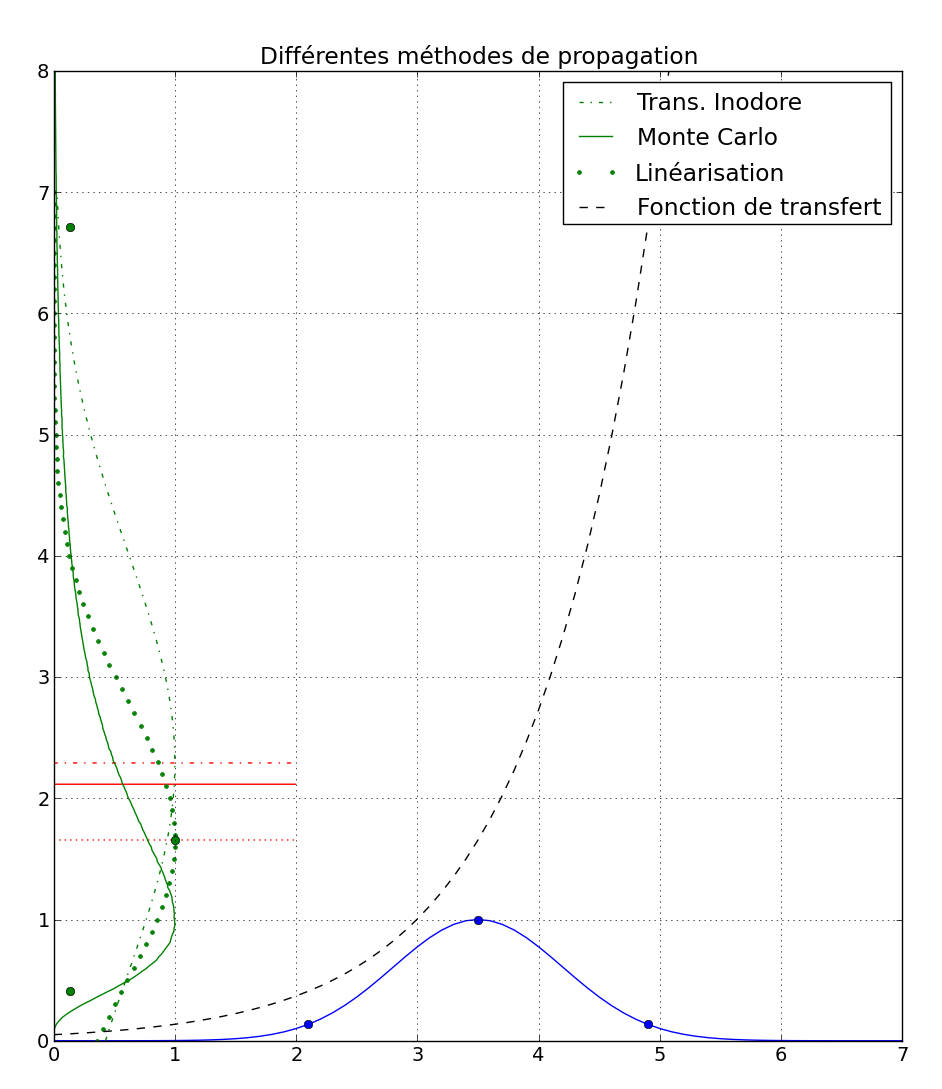
\includegraphics[width=0.7\textwidth]{Chapter4/graphics/unscented_transform.png}
	\caption{Illustration de différents procédés de propagation d'une variable aléatoire. La courbe bleue représente la distribution initiale. Les courbes vertes représentent les distributions propagées, de manière exacte (continue) ou approximatives. Les lignes rouges représentent les valeurs moyennes estimées de la variable propagée}
	\label{fig:ch4_transformation_evaluation}
\end{figure}

\subsubsection{Remarques:}
Plusieurs éléments sont à remarquer sur la Figure \ref{fig:ch4_transformation_evaluation}, très dense en informations. La transformation utilisée étant non-linéaire et non-symétrique par rapport à la valeur moyenne de la variable initiale, la distribution de la variable aléatoire dans l'espace d'arrivée est fortement dissymétrique, elle ne correspond pas à une gaussienne (son troisième moment statistique, le \og \emph{skew}\fg{}, n'est pas nul. Ce troisième moment est par construction nul pour une loi normale). On peut remarquer que l'usage de la transformée inodore permet de capturer une partie de cette dissymétrie (les points sigma ne sont pas non plus symétriques dans l'espace d'arrivée), mais l'estimation d'une gaussienne à partir de ces points perd cette information. La transformée inodore inverse consiste en effet à calculer les deux premiers moments modélisés par les points sigma. Dans cet exemple (les performances des différentes approches varient avec la transformation choisie, notre cas n'en est qu'une illustration), les paramètres estimés sont présentés dans le tableau \ref{tab:ch4_comparaisons_linéarisation}.

\subsubsection{Quelques résultats:}
On recense dans le tableau \ref{tab:ch4_comparaisons_linéarisation} les résultats des estimations des deux premiers moments statistiques de la variable propagée, selon les méthodes de linéarisation et de transformation inodore. On pourra retenir que la linéarisation est efficace si la variance de l'état d'entrée est faible devant la non-linéarité de la fonction approximée, mais qu'elle peut être mise en défaut quand la variance s'accroît. Dans cet exemple (le plus souvent, d'après Julier ou Kraft \cite{Julier1997, Kraft2003}), la linéarisation de la transformation conduit à une sous-estimation de la variance, ce qui peut être problématique dans le cas d'un filtre. \\

On peut comprendre ce phénomène assez simplement : on suppose dans cette approximation que la pente de la transformation est constante, mesurée au niveau de la moyenne de la variable initiale. Dans notre cas, cette pente est très inférieure à celle à laquelle est potentiellement soumise la variable sur l'ensemble de ses valeurs probables. La covariance de l'état de sortie est alors sous-estimée. L'inverse est bien sûr possible, si la pente de la transformation est maximale au niveau de la valeur moyenne. L'efficacité de la linéarisation opérée dans le filtre EKF est donc relative à la variance de l'état propagée \textit{et} à la linéarité initiale de la fonction de transfert, tandis que cette dernière est souvent la seule prise en compte intuitivement. Le problème de la sous-estimation de la variance propagée est souvent mitigé en pratique par l'ajout d'un bruit constant ($R$ dans l'équation \ref{eq:EKF_pred2}).

\begin{figure}
	\begin{equation}
	\begin{array} {| c | c | c |}
	\hline
	& & \\
	\textnormal{\emph{Procédé}} & \textnormal{\emph{Moyenne}} &	\textnormal{\emph{Écart-type}}\\
	\hline
	& & \\
	\textnormal{Monte-Carlo	(exact)}	& 2.12  &	1.68 \\
	\hline
	& & \\
	\textnormal{Linéarisation} & 1.66	& 1.16 \\
	\hline
	& & \\
	\textnormal{Transformation inodore}	& 2.29	&	1.76 \\
	\hline
	\end{array}	
	\end{equation}
	\caption{Quelques chiffres illustrant les différents procédés}
	\label{tab:ch4_comparaisons_linéarisation}
\end{figure}


\section{Algorithme proposé}
Dans le cadre de notre application, nous devons être capables de suivre dans le temps et de positionner le plus de points possibles, afin d'augmenter la densité de l'échantillonnage de la scène et ainsi de pouvoir détecter d'éventuels obstacles. Nous proposons donc une approche (\cite{Lefaudeux2012}) dissociant l'estimation du mouvement de celle de la position des points, similaire en cela à la proposition faite dans l'algorithme \emph{PTAM} (\cite{Klein2007}). Ces deux problématiques sont intrinsèquement liées, et il semble \textit{a priori} relativement naturel d'en lier la résolution. Toutefois, cela limite en pratique le nombre de points que nous sommes capables de positionner simultanément. En outre, les contraintes de précision sur l'estimation du mouvement et sur la position des éléments détectés sont dans notre cas bien distinctes, la seconde n'étant pas nécessairement très grande. Enfin, l'exhaustivité des informations disponibles au sortir de notre étape de suivi de points, qui est à la fois plus robuste (du fait du mécanisme de rejet des points non fiables) et plus dense que la plupart des approches présentes dans la littérature présentant un SLAM visuel, nous assure un résultat satisfaisant. La détermination de l’ego-motion en est grandement simplifiée, et l'approche que nous proposons, bien qu'assez simple au regard d'autres stratégies possibles, est suffisamment précise pour nos besoins tout en étant très rapide.

\subsection{Détermination de l'Ego-Motion}
\subsubsection{Transformation rigide à partir de nuages de points appariés} \label{sec:ch4_ego_motion}
% suite à nos observations visuelles, et des correspondances entre chacun de ces points. La mise en correspondance de points entre deux plans image dont les référentiels relatifs sont connus se traduit ainsi en une position dans l'espace du point observé, par rapport à l'un de ces référentiels, et notre suivi de points dans le temps nous fournit ces correspondances. Il est alors possible d'utiliser une des nombreuses méthodes proposées au paragraphe précédent, qui n'utilisent pas ces nuages de points connectés, ou bien de se rapprocher des techniques développées à cet effet, le plus souvent en dehors du cadre spécifique de la stéréovision. \\

On dispose tout d'abord de deux nuages de points issus de notre paire stéréoscopique, et mis en correspondance (Chapitre 3). Le suivi des points entre les deux caméras permet de les traduire en autant de positions en trois dimensions (cf. \ref{sec:ch2_Modèle Stéréovision}), tandis que le suivi dans le temps assure une correspondance point-à-point des deux nuages obtenus. Ce suivi dans le temps est important, car il nous évite d'appliquer les algorithmes de filtrage et d'optimisation classiques (par exemple de type \textit{ICP}). Il est ainsi possible de rechercher directement la transformation rigide permettant de passer d'un nuage de points à un autre.\\
Nous avons retenu une méthode par décomposition en éléments propres pour estimer initialement la transformation. Cette méthode n'est pas utilisée tel quel, l'estimation obtenue dans un cadre de stéréo-vision et dans un environnement contenant des objets mobiles ou mal appariés n'étant pas satisfaisante. Nous en proposons au paragraphe suivant une application itérative et par pondération qui permet d'obtenir des performances satisfaisantes pour notre application, à un coût calculatoire très faible.\\

L'approche de Bak (section \ref{ch4:méthode_bak}), est très intéressante dans notre problématique, et très exactement adaptée à l'estimation du mouvement par un système de stéréo-vision. Cependant le système dans cette méthode est $O(N^2)$, ce qui limite le nombre de points pouvant être pris en compte (à temps de calcul donné), ou encore le nombre d'itérations possible pour estimer de manière robuste les points aberrants (cf. \ref{sec:ch4_robust_estimation}). Nous avons considéré, au vu des résultats obtenus par une approche moins optimale mais itérée et pondérée (\ref{sec:ch4_eval_ego_motion}), que la prise en compte robuste des points aberrants était satisfaisante.

\paragraph{Méthode par décomposition en éléments propres:\\} \label{sec:ch4_estimation_transformation_rigide}
On détaille ici l'une des méthodes utilisées pour estimer le mouvement entre deux acquisitions, lorsque l'on dispose de plusieurs caméras dont la configuration spatiale est connue. La méthode que nous proposons (section \ref{sec:ch4_ego_motion}) reprend beaucoup d'éléments d'une approche de l'état de l'art, dite \og SVD\fg{} (\emph{Singular Value Decomposition}, Décomposition en Éléments Propres).\\

La connaissance de la correspondance entre plusieurs points d'un nuage ayant subi une transformation géométrique rigide rend possible l'estimation très rapide de cette transformation, ce problème étant par ailleurs connu depuis plusieurs décennies, sous le nom du problème de \emph{Procuste}. \footnote{Ce nom fait référence au bandit de la mythologie grecque, qui parvenait tant bien que mal à adapter ses victimes à la taille de son lit. La transformation nécessaire était appliquée de manière quelque peu sommaire (par la coupe des pieds de sa victime). La correction à appliquer était dans ce cas maximisée par l'utilisation de deux modèles de lit différents, de sorte que les victimes ne soient jamais dans un lit adapté. Ce nom est resté pour s'appliquer à de nombreux problèmes liés à une estimation d'échelle ou de transformation rigide. Il est souvent utilisée sous sa forme originale (Procruste) dans la littérature anglo-saxonne, tandis que la littérature francophone utilise le nom Procuste.} Il existe au moins 4 approches répondant à ce problème, détaillées dans \cite{Eggert1997}. Les deux premières approches sont similaires, et paramètrent la transformation rigide de manière matricielle. On cherche alors à minimiser l'erreur moyenne dans la norme $L_2$. Deux autres méthodes sont proposées, modélisant la transformation rigide par des quaternions, qui ont la propriété de ne pas être soumis aux singularités présentes dans les rotations telles que représentées par des matrices. La minimisation de l'erreur est dans tous les cas obtenue par une décomposition en éléments propres d'une matrice de corrélation, de dimension très réduite. \\

Cette méthode est très utilisée dans le domaine du recalage de nuages de points obtenus par télémètre laser, au travers de l'algorithme \emph{ICP} dont elle constitue l'une des étapes. Elle est par ailleurs très facilement exploitable de part son caractère matriciel et linéaire, et son temps d'exécution varie peu en fonction du nombre de points utilisés. L'erreur minimisée dans cette procédure n'est cependant pas exactement adaptée aux problématiques de la stéréo-vision, et nous en proposons dans \ref{sec:ch4_robust_estimation} un usage itératif et pondéré qui la rend plus robuste et plus fiable dans ce contexte. \\

Sa présentation initiale est le fait de Arun (\cite{Arun1987}), un cas de rotation problématique ayant ensuite été précisé par Umeyama \cite{Umeyama1991}. Les notations employées par la suite sont celles de \cite{Eggert1997}. Considérons les nuages de points ${m_i}$ et ${n_i}$ ($i=1,..,N$), et la transformation recherchée (composée d'une rotation et d'une translation) $[\hat{R}, \hat{T}]$ qui permet de recaler les deux nuages de points. Ceci équivaut à minimiser l'erreur $\Sigma$ telle que :

\begin{equation} \label{eq:ch4_l2_norm}
\Sigma^2 = \sum\limits_{i=1}^{N} {\| n_i - \hat{R} m_i - \hat{T} \|}^2
\end{equation}

On suppose ici une correspondance parfaite entre les nuages dans le jeu de données, et un bruit isotrope et uniforme sur la position de chacun des points (ces deux caractéristiques étant discutées par la suite). L'estimation de la rotation et de la translation peut être faite en deux temps, par le biais de la position moyenne de chacun des nuages de points. On ramène chacun des nuages à son centre de masse pour estimer la rotation permettant de ramener les deux nuages dans le même référentiel. On calcule les centres de masse $\overline{m}$ et $\overline{n}$:

\begin{align}
	\begin{split}
		\overline{m} =& \frac{1}{N} \sum\limits_{i=1}^{N} m_i \\
		\overline{n} =& \frac{1}{N} \sum\limits_{i=1}^{N} n_i
	\end{split}
\end{align}

puis les vecteurs ${m_c}$ et ${n_c}$ décrivant les points relativement à leur centre de masse respectifs :

\begin{align}
	\begin{split}
		{m_c}_i =& m_i - \overline{m} \\
		{n_c}_i =& n_i - \overline{n}
	\end{split}
\end{align}

L'équation \ref{eq:ch4_l2_norm} s'écrit alors :

\begin{align} \label{eq:ch4_eq_to_minimize}
	\begin{split}
		\Sigma^2 =& \sum\limits_{i=1}^{N} {\| {n_c}_i - \hat{R} {m_c}_i \|}^2 \\
		=& \sum\limits_{i=1}^{N} {{n_c}_i}^T {n_c}_i + {{m_c}_i}^T {m_c}_i - 2 {{n_c}_i}^T \hat{R} {m_c}_i
	\end{split}
\end{align}

Les termes liés au produit scalaire de ${n_c}_i$ et ${m_c}_i$ étant constants, la minimisation de $\Sigma^2$ conduit donc à maximiser ${{n_c}_i}^T \hat{R} {m_c}_i$. On introduit pour ce faire la matrice $H$, matrice de corrélation, définie par :

\begin{equation}
H \stackrel{def}{=} \sum\limits_{i=1}^{N} {{m_c}_i}^T {n_c}_i
\end{equation}

On pourra remarquer que cette matrice est de dimension 3x3, quelque soit la taille du nuage de points. Minimiser l'équation \ref{eq:ch4_eq_to_minimize} est alors équivalent à maximiser la trace $Tr(\hat{R} H)$. Une solution pour maximiser $Tr(\hat{R} H)$ consiste à utiliser la décomposition en éléments propres de $H$, que l'on note traditionnellement $H = U \Lambda V^T$. $U$ et $V$ sont ici des matrices de passage, orthogonales ($V^{-1} = V^T$), tandis que $\Lambda$ est une matrice diagonale contenant les valeurs propres de $H$. La matrice maximisant la trace désirée est alors :

\begin{equation}
\hat{R} = V U^T
\end{equation}

On obtient finalement la translation nécessaire à l'alignement des nuages $m_i$ et $n_i$ par la distance entre les centres de masse après application de la rotation estimée :

\begin{equation}
\hat{T} = \overline{n} - \hat{R} \overline{m}
\end{equation}

Umeyama (\cite{Umeyama1991}) a toutefois montré que cette procédure pouvait conduire à une rotation estimée inversée, et en a proposé une correction très simple. Si le produit $det(U) \cdot det(V)$ est négatif, $\hat{R}$ devient égale à $V S U^T$ avec $S$ une matrice diagonale $diag(1,1,..., 1, -1)$. \\

Plusieurs limitations sont cependant à soulever quant à l'utilisation de cette procédure pour calculer l’ego-motion avec un dispositif de type stéréo-vision. On suppose tout d'abord que les deux nuages de points sont \og parfaits\fg{}, c'est-à-dire que l'on ne prend ni bruit ni erreur d'appariement en compte. Goryn et Hein (\cite{Goryn1995}) ont montré que cette solution était conservée en présence de bruit de moyenne nulle, mais cela ne prend pas en compte d'éventuelles erreurs d'appariement. On recherche par ailleurs la transformation rigide optimale entre ces deux nuages de points, mais ceux-ci peuvent contenir des objets mobiles, dont le déplacement ne peut alors pas être modélisé par un couple rotation-translation. On détaillera dans \ref{sec:ch4_robust_estimation} l'algorithme proposé pour se prémunir de ces deux sources d'erreur possibles. 

\subsubsection{Estimation robuste et détermination des outliers} \label{sec:ch4_robust_estimation}
La méthode par décomposition en éléments propres calcule la transformation rigide minimisant l'erreur dans la norme $L_2$ de recalage de deux nuages de points. Nous avons vu que cela n'était pas nécessairement optimal dans le cas de nuages de points issus d'un dispositif de stéréo-vision, et que cette formulation n'était pas robuste aux points marginaux correspondant par exemple aux éléments en mouvement de la scène. On propose donc une amélioration de cette méthode, qui nous permettra d'appliquer des principes de pondération et de calcul itératif présents dans les calculs robustes de statistiques. Ceux-ci sont sommairement introduits en annexe (\ref{sec:Annexe_robust}), une présentation plus complète étant hors de portée dans le cadre de ce manuscrit. Les positions des points utilisées dans le nuage \textit{passé} sont, lorsque cela est possible (si ce point a été observé plusieurs fois consécutivement), des positions filtrées. Ce filtrage est détaillé dans \ref{sec:ch4_filtrage_nuage}.

\paragraph{Pondération de la méthode \og SVD\fg{}:\\} \label{sec:ch4_svd_pondérée}
On propose tout d'abord de conserver la minimisation d'une fonction de coût basée sur la norme $L_2$, telle que présentée dans l'équation \ref{eq:ch4_l2_norm}. Ceci nous permet en effet de conserver la résolution à base de SVD très rapide, et commode de part sa complexité faible par rapport au nombre de points prise en compte. On propose cependant d'y associer une pondération individuelle déterminée de manière robuste, afin de mieux prendre en compte la fiabilité de chacun des points. On note ${n_c}_i$ et ${m_c}_i$ les coordonnées des points du premier et du second nuage respectivement, centrées par rapport à leur centre de masse respectif et $N$ le nombre de points. La valeur que l'on cherche à minimiser devient alors, en supposant que l'on puisse identifier une pondération $\alpha$ efficace:
\begin{align} \label{ch4:eq_to_minimize_weighted}
	\begin{split}
		&\forall_i \in [1,N], \: \alpha_i \in R_{+}^{*} \\
		&\Sigma^2 = \sum\limits_{i=1}^{N} \alpha_i {\| {n_c}_i - R {m_c}_i \|}^2 \\
		&\hat{R} = \min_R \Sigma^2
	\end{split}
\end{align}
Comme précédemment, cela est équivalent à maximiser la trace (en utilisant les propriétés de symétrie de la matrice de rotation recherchée)
\begin{equation} \label{ch4:trace_maximize}
Tr(\hat{R} \cdot (\sum\limits_{i=1}^{N} \alpha_i \; {{m_c}_i}^T \cdot {n_c}_i ))
\end{equation}

ce qui nous permet d'introduire la nouvelle matrice de corrélation $H_\alpha$ :
\begin{equation}
	H_\alpha \stackrel{def}{=} \sum\limits_{i=1}^{N} { \alpha_i \; {m_c}_i}^T \cdot {n_c}_i
\end{equation}

On peut alors reprendre un lemme, notamment dérivé dans \cite{Arun1987}, stipulant que pour toute matrice $AA^T$ définie positive, pour toute matrice $B$ orthonormale:
\begin{equation}
	Trace(AA^T) \geq Trace(BAA^T)
\end{equation}

La démonstration utilisée dans le cas classique d'une matrice $H$ non pondérée s'applique ici, à condition que la matrice $H_\alpha$ soit bien de rang 3. Les coefficients $\alpha_i$ étant positifs et non tous nuls, il suffit que les vecteurs $n_i$ et $m_i$ ne soient pas tous simultanément orthogonaux pour garantir le rang de $H_\alpha$. Ceci est évité avec des points non coplanaires, ce qui n'est pas vraiment contraignant en pratique. On peut donc proposer une décomposition en éléments propres de $H_\alpha$, dénotée par :
\begin{equation}
	H_\alpha = U \Lambda V^T
\end{equation}
avec $U$ et $V$ des matrices orthonormales 3x3 (matrices de passage) et $\Lambda$ la matrice diagonale 3x3 des valeurs propres. En multipliant $H_\alpha$ par la matrice $X = VU^T$, orthonormale ($U$ et $V$ étant orthonormales), de sorte que :
\begin{align}
	\begin{split}
		X H_\alpha	&= V U^T U \Lambda V^T \\
			&= V \Lambda V^T
	\end{split}
\end{align}

$XH_\alpha$ est donc définie positive de taille 3x3, ce qui implique, avec le lemme précédent, que pour toute matrice B orthonormale de taille 3x3 :
\begin{equation}
	Tr(X H_\alpha) \geq Tr(B X H_\alpha)
\end{equation}

La matrice X proposée maximise bien la trace voulue, et nous fournit alors la matrice orthogonale minimisant l'équation \ref{ch4:eq_to_minimize_weighted}.

\paragraph{Recherche itérative:\\} \label{sec:ch4_iterative_ego_motion}
Il s'agit maintenant de proposer une pondération pertinente de chacune des contributions à la matrice de corrélation $H_\alpha$. On se base pour cela sur le domaine dit des \og statistiques robustes\fg{}, présenté au moins partiellement en annexe (cf. section \ref{sec:ch4_estimateurs_robustes}). Contrairement à la méthode retenue pour un RANSAC (\cite{Fischler1981}), on choisit dans notre approche de se baser sur une pondération itérative des différentes contributions à la matrice $H_\alpha$, pour deux raisons : on ne sait \textit{a priori} pas quels seront les points fiables parmi les milliers de points suivis (une sélection aléatoire sur l'ensemble des points serait coûteuse en temps de calcul), et on suppose que les points sont majoritairement corrects, justifiant une approche plus déterministe. Une représentation schématique du processus suivi est visible sur la figure \ref{fig:ch4_estimation_ego_motion}. L'algorithme proposé pour déterminer le mouvement peut s'écrire :

\begin{enumerate}
	\item {\emph{Initialisation}}\\
	La contribution de chacun des points à la matrice $H_\alpha$ est pondérée par l'inverse de la distance entre le plan image et ce point, poids initial en accord avec une modélisation rapide du bruit d'un nuage de points issu de stéréo-vision (cf. \ref{sec:ch2_Modèle Stéréovision}). On pourra remarquer qu'il s'agit également de la covariance initiale des points dans le modèle proposé par Montiel \textit{et al.} (\cite{Montiel}), SLAM visuel très largement utilisé. La distance est seuillée pour éviter toute singularité (et une trop forte confiance dans les points proches).
	\begin{equation}
		\alpha_{i,0} = \frac{1}{min(d_i, d_{min})}
	\end{equation}

	\item {\emph{Itérations}}
	\begin{itemize}
		\item{\textbf{Calcul de la transformation}}\\
		À l'itération $k$, la transformation est calculée avec les poids ${\alpha_{i,k}}k$ et par une décomposition en éléments propres, comme présenté dans \ref{sec:ch4_svd_pondérée}. Cette étape prend en compte l'intégralité des points suivis, mais reste extrêmement rapide du fait de l'accumulation mise en œuvre.\\
		
		\item{\textbf{Actualisation des poids}}\\
		On calcule, tout d'abord, des indicateurs robustes décrivant la distribution des points après recalage. On considère ici les estimateurs médiane (cette dernière étant calculée par l'algorithme de Hoare connu sous le nom de \emph{Quick Select}, de complexité linéaire) et MAD (\ref{eq:ch4_MAD}), que l'on note ci-dessous $\mu_{median,k}$ et $\sigma_{MAD,k}$. Ces estimateurs s'appliquent sur l'erreur de position entre les deux observations d'un même point, ramenées dans un même référentiel. La statistique est alors effectuée sur l'ensemble du nuage. \\
		On calcule ensuite les nouveaux poids $\alpha_{i,k+1}$ , en utilisant une fonction $\rho$ qui est dérivée de la fonction de Tukey \emph{biweight} (\cite{Huber1981}, voir par ailleurs section \ref{sec:Annexe_robust}).
		\begin{align}
			\begin{split}
				\forall i \in [1,N], d_{i,k}^2 &= \| {n_c}_{i,k} - \hat{R}_k {m_c}_{i,k}\|^2 \\
				\delta &= \frac{\lvert d_i - \mu_{median, k}\rvert}{\sigma_{MAD, k}} \\
				\alpha_{i,k+1} &= \rho(\delta)
			\end{split}
		\end{align}
		La variable $\delta$ correspond à l'erreur de recalage du point considéré, c'est-à-dire à la distance résiduelle sur ce point après avoir appliqué sur le premier nuage la rotation $R_k$. Cette erreur est relative à l'erreur médiane sur le nuage, et à sa dispersion. La fonction de coût $\rho$ est celle dite de \emph{Tukey Biweight} sur $\mathbb{R}^+$, et 0 sur $\mathbb{R}^-$.\\
		
		\item{\textbf{Test de la condition d'arrêt}}\\
		Trois critères sont utilisés pour continuer ou non les calculs : le nombre d'itérations maximal $k_max$ (on souhaite travailler en temps de calcul borné), la qualité du recalage des nuages de points (par rapport à une erreur médiane souhaitée $\mu_{min]}$) et l'amélioration obtenue après la dernière itération (avec $r_min$ décrivant le ratio d'amélioration du recalage en deçà duquel les itérations sont arrêtées):
		\begin{align}
			\begin{split}
				k &< k_{max} \\
				\mu_{median} &> \mu_{min} \\
				\frac{\lvert \mu_{median, k} - \mu_{median, k-1} \rvert}{\mu_{median, k}} &> r_min
			\end{split}
		\end{align}\\
	\end{itemize}
\end{enumerate}

\begin{figure}
	\centering
	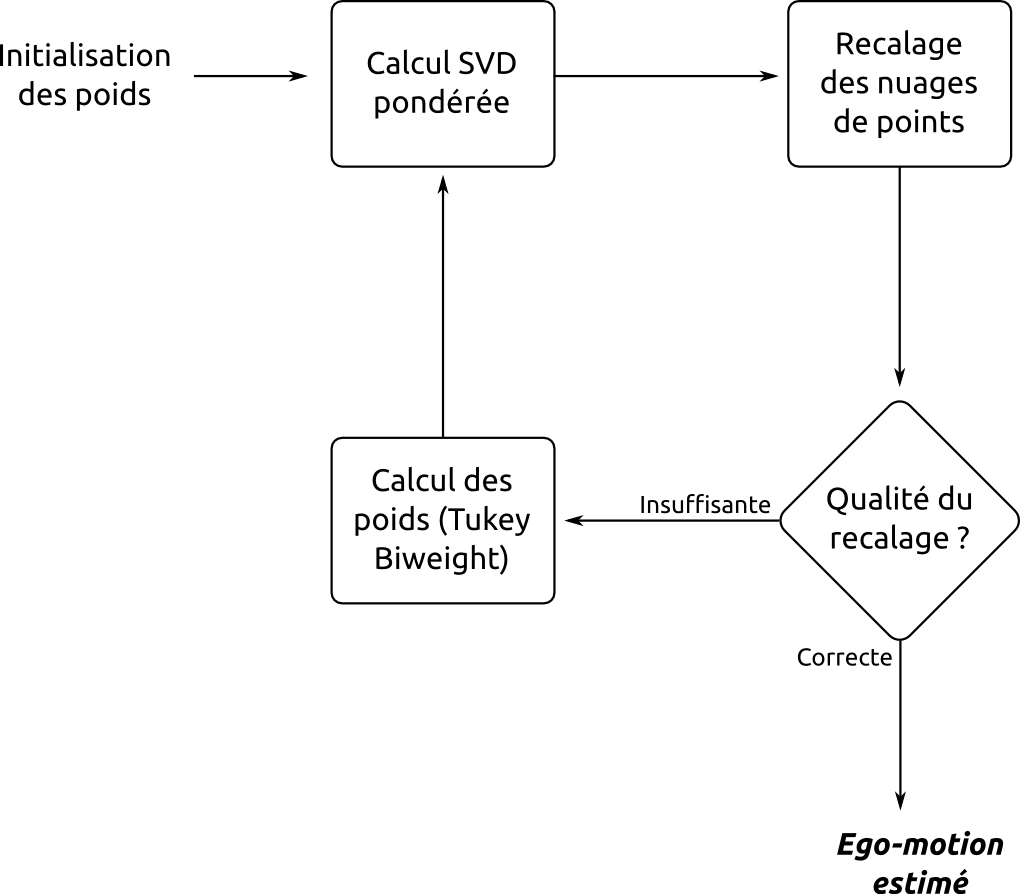
\includegraphics[width=0.7\textwidth]{Chapter4/graphics/overall_scheme_ego.png}
	\caption{Algorithme proposé pour estimer l'\textit{ego-motion} à partir des nuages de points}
	\label{fig:ch4_estimation_ego_motion}
\end{figure}

\subsubsection{Filtrage de l'ego-motion par UKF}
\paragraph{Pourquoi filtrer ?\\}
L'estimation de l'ego-motion présentée dans \ref{sec:ch4_robust_estimation} consiste en une optimisation locale, dans le sens où elle ne prend en compte que les deux dernières acquisitions pour calculer le déplacement. Nous avons vu précédemment (section \ref{sec:ch4_state_of_art_VO}) que plusieurs méthodes étaient possibles. Une optimisation sur plusieurs acquisitions consécutives \cite{Nister2006, Lategahna, Konolige2008} est une possibilité, mais il est également possible d'envisager un filtrage de nos observations pour obtenir la prise en compte de notre historique de mesure dans chaque nouvelle estimation (cf. figure \ref{fig:ch4_pourquoi_filtrer}). Nous retrouvons ici la dualité filtrage/optimisation présente dans de nombreuses approches de SLAM. Dans l'hypothèse où notre système est Markovien de rang 1 (hypothèse forte qui n'est pas nécessaire pour une approche d'optimisation multi-acquisitions), la littérature consacre de nombreux filtres à même d'estimer un ego-motion optimal.\\

Il s'agit de l'approche que nous avons retenue, du fait de la légèreté des nombreux filtres disponibles, de son intégration efficace dans un environnement multi-capteurs, et des performances obtenues qui nous ont semblé suffisantes. Une approche par optimisation est toujours possible, et serait peut-être à développer dans des travaux futurs, notamment en fonction de la puissance de calcul disponible sur la plate-forme embarquée choisie.\\

Il ne s'agit pas ici de réaliser un état de l'art des différents algorithmes de filtrage présents dans la littérature, tant ceux-ci sont nombreux et complexes. On introduit cependant dans les prochains paragraphe la solution que nous avons retenue, tout en présentant quelques éléments de choix qui ont prévalu.

\begin{figure}
	\centering
	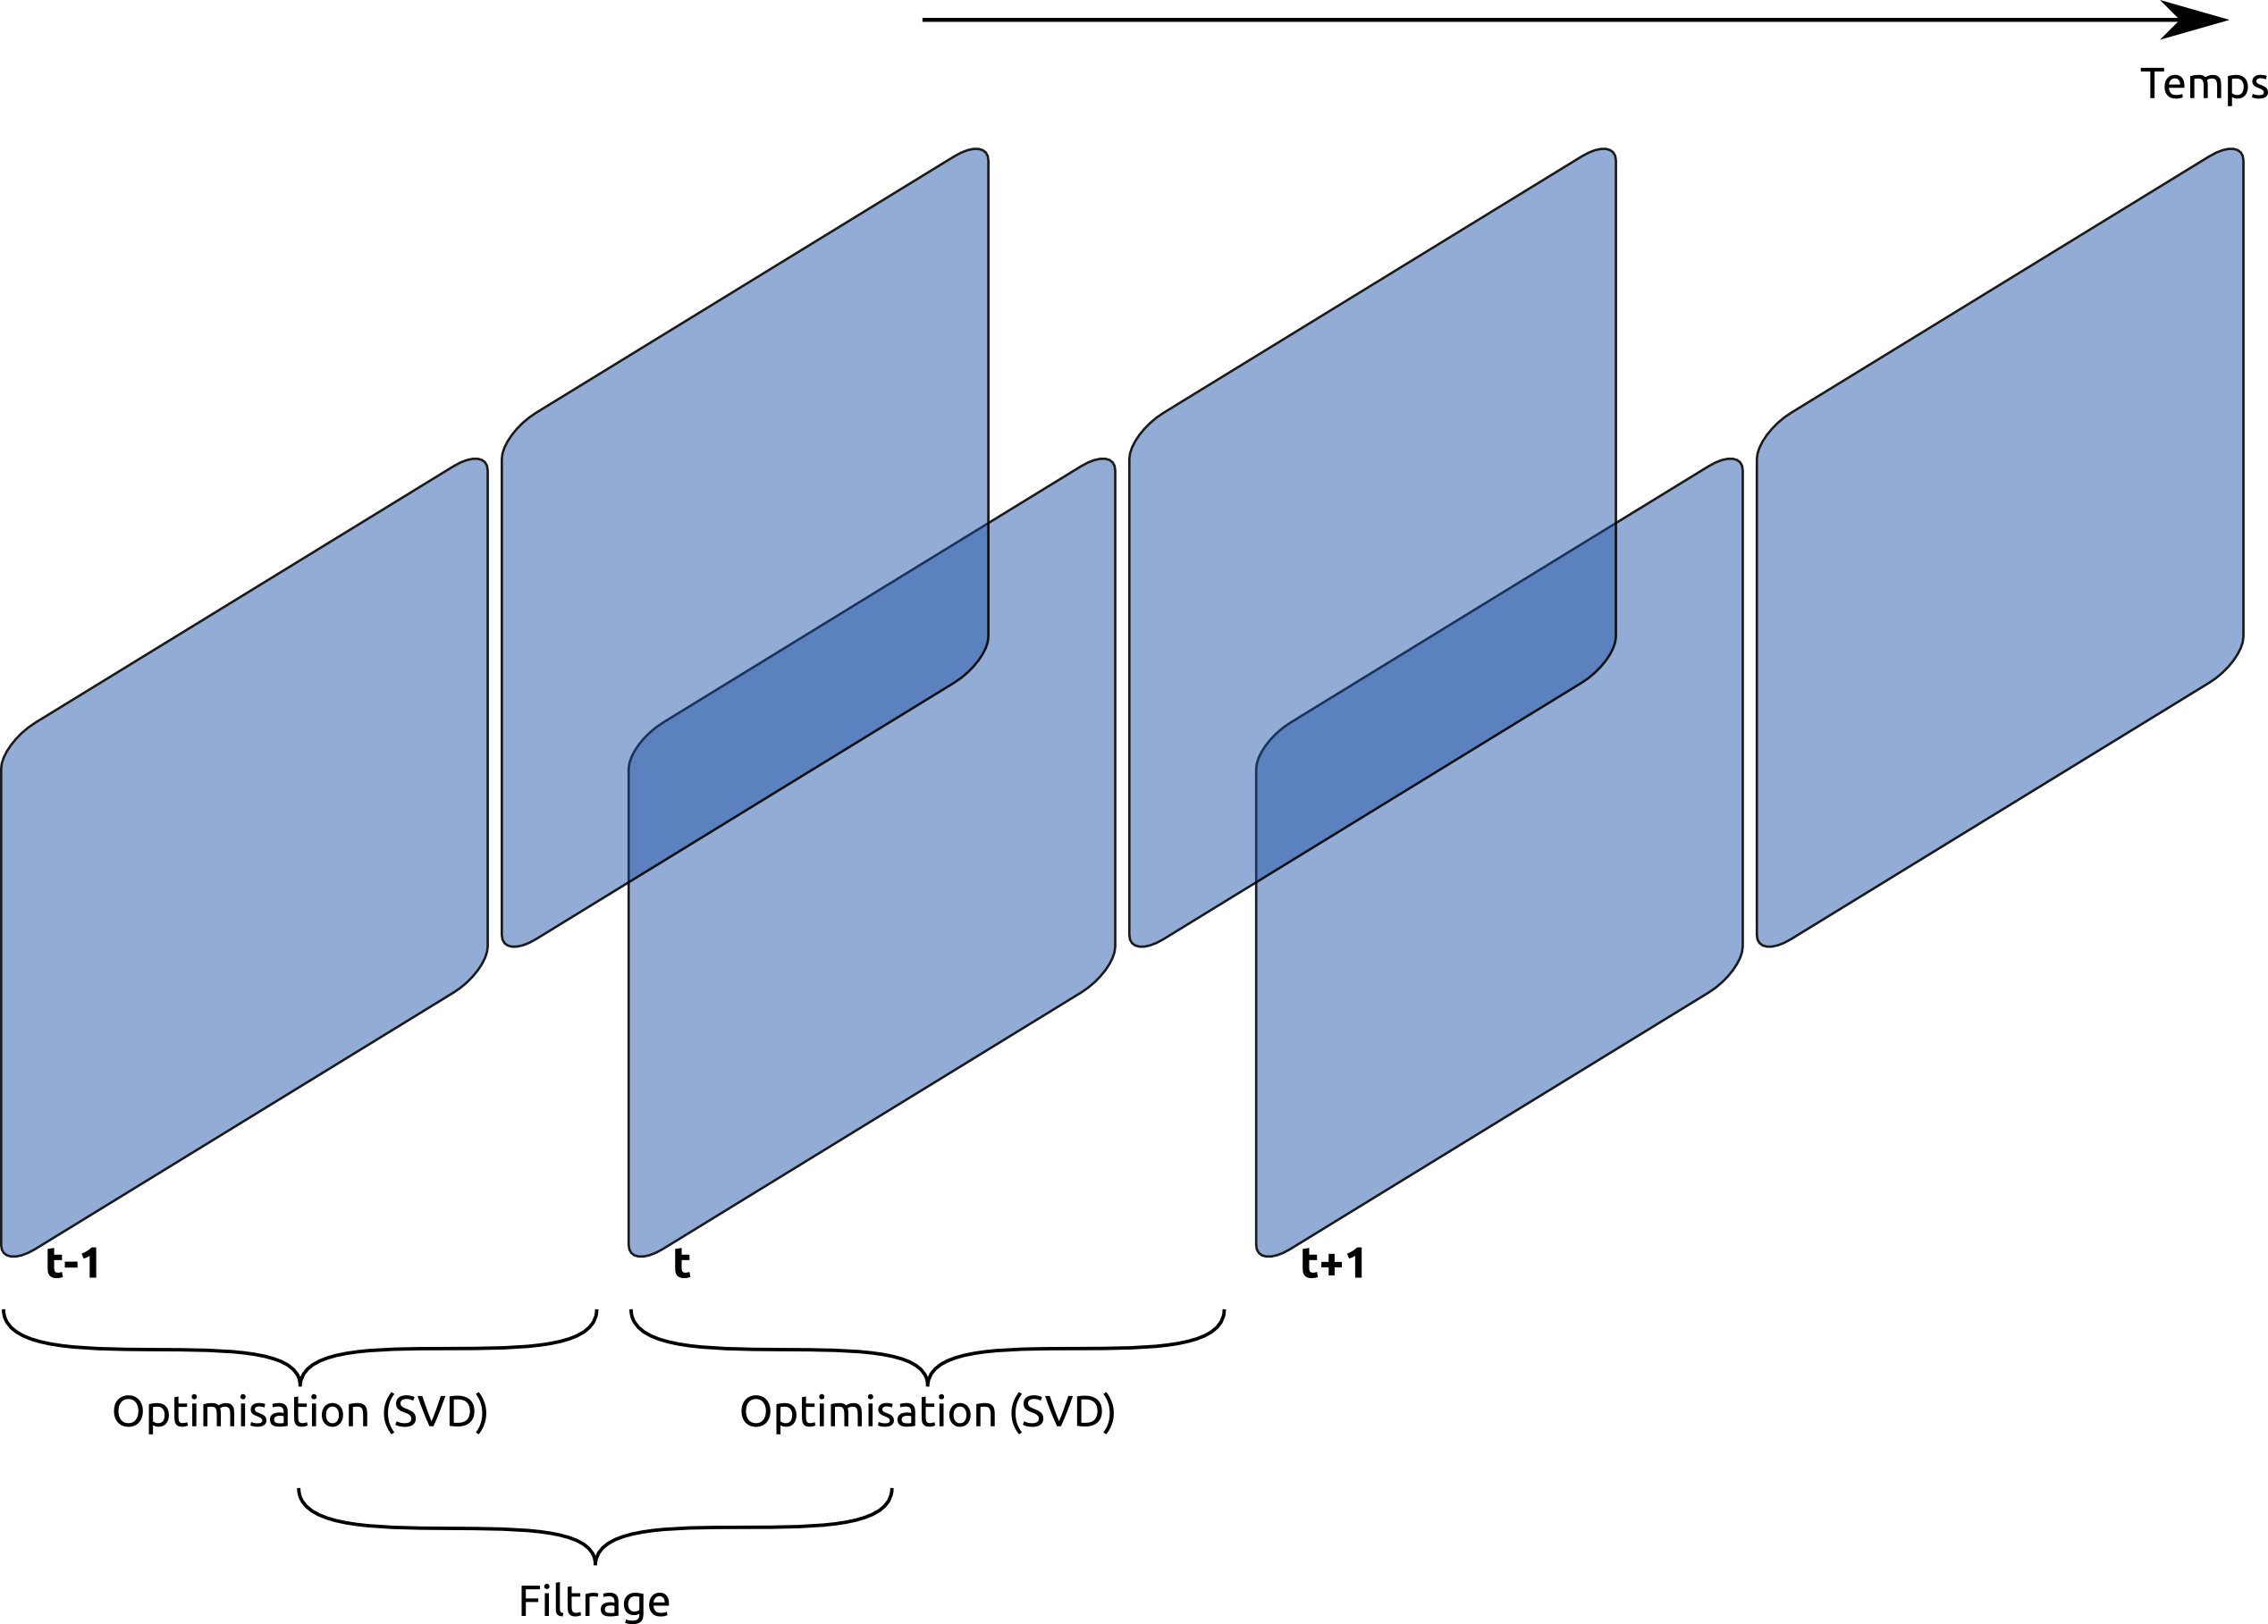
\includegraphics[width=0.8\textwidth]{Chapter4/graphics/why_filter.png}
	\caption{Illustration de l'apport du filtrage en termes de nombre d'acquisitions prises en compte}
	\label{fig:ch4_pourquoi_filtrer}
\end{figure}

\paragraph{Quel type de filtre choisir ?\\}
Comme nous l'avons détaillé dans \ref{sec:ch4_filtrage}, de nombreux algorithmes de filtrage sont présents dans la littérature, parmi lesquels le filtre de Kalman et quelque unes de ses variantes. Celui-ci est tout d'abord limité à des fonctions de propagation et de mesure linéaires, ce qui est en pratique très contraignant dans de nombreuses utilisations. L'estimation de la position courante à partir d'odométrie visuelle couplée à un système GPS ou à une centrale inertielle implique par exemple des fonctions non-linéaires lors des changements de référentiel. La fusion de données de positions relatives dans le cadre d'une collaboration entre véhicules est un autre exemple de mesure potentiellement non-linéaire.\\

Nous n'avons pas mis en œuvre de tel couplage dans le cadre de cette thèse, mais avons néanmoins choisi d'implémenter une solution l'autorisant dans un avenir proche. Ceci implique donc d'envisager les extensions EKF et UKF au filtre de Kalman, toutes deux capables de prendre en compte des fonctions de mesure linéarisables.\\

L'estimation de la position angulaire est ensuite rendue complexe par des singularités, si les angles sont paramétrés par les angles d'Euler. Les quaternions (introduits dans la section suivante) offrent une représentation plus simple à cet égard, et leur implémentation est rendue plus facile dans un UKF de par les points Sigma et l'absence du calcul de Jacobien (voir notamment \cite{Kraft2003}).\\

Nous avons choisi de nous concentrer sur le filtre de Kalman inodore, pour sa (relative) simplicité dans la gestion de fonctions de mesure et de propagation fortement non-linéaires, et ses performances supérieures à l'EKF dans ces cas de figure. 

\paragraph{Filtrage par Kalman inodore:\\}
Nous avons donc implémenté un algorithme de type UKF, avec un modèle de mouvement à vitesse constante (qui ne tient donc pas compte du mouvement non-holonomique des véhicules roulants usuels). Ce filtre utilise une représentation des angles par quaternions, qui permet de se prémunir simplement des singularités présentes dans une représentation eulérienne. Les quaternions sont une extension des nombres complexes classiques (qui autorisent notamment le paramétrage d'une rotation dans un plan), présents dans l'ensemble $\mathbb{H}$ homogène à $\mathbb{R}^4$, souvent représentés par leurs éléments de base \emph{(1,i,j,k)}, qui vérifient :

\begin{align}
	i^2 &= j^2 = k^2 = ijk = -1 \\
	q &= q_0 + q_1 \cdot i + q_2 \cdot j + q_3 \cdot k \qquad | \qquad \{q_k\}_{k \in [0..3]} \in \mathbb{R}
\end{align}

Les quaternions représentant une rotation sont restreints à $\mathbb{H}_1$, qui décrit les quaternions unitaires :

\begin{equation}
	\lVert q \rVert = \sqrt{q_0^2 + q_1^2 + q_2^2 + q_3^2} = 1
\end{equation}

La représentation des rotations en trois dimensions dans l'espace des quaternions unitaires ne souffre pas de singularités, ce qui simplifie grandement les étapes de propagation ou de mise à jour de l'estimation angulaire. La génération des points sigma de la transformation inodore est cependant un peu plus complexe, un exemple de procédé étant par exemple décrit dans \cite{Kraft2003}. \\
On pourra retenir que cette représentation n'est pas à proprement parler nécessaire dans le cas d'un filtrage du mouvement seul, les vitesses angulaires n'étant \textit{a priori} jamais proches des points $\pi$ ou $-\pi$. Cette représentation devient cependant très commode dès lors que l'on couple notre estimation avec un capteur de position angulaire, et que l'on cherche à estimer la position courante.


\subsection{Filtrage du nuage de points statiques échantillonné dans le temps} \label{sec:ch4_filtrage_nuage}
\subsubsection{Matrice de visibilité} \label{sec:ch4_matrice_visibilité}
On définit tout d'abord une matrice de visibilité, permettant de gérer les apparitions et disparitions successives des points observés. On se place ici dans une approche différente de la plupart des techniques présentées précédemment : l'enjeu, pour nous, est d'être capable de gérer en temps réel un nombre sensiblement constant de points d'intérêt répartis sur l'image, afin d'être à tout moment capable de détecter d'éventuels obstacles. La matrice de visibilité nous permet de rendre compte de l'observabilité des points lors des acquisitions successives, un point perdu lors d'une étape de suivi n'étant par ailleurs jamais réintroduit sous la même forme. La visibilité $V_{i,k}$ du point $i$ lors de l'acquisition $k$ vaut 1 lorsque ce point est le même que lors de l'acquisition $k-1$. S'il est perdu au cours de l'acquisition $k$, $V_{i,k}$ vaut 0 et un nouveau point est introduit avec la procédure décrite dans \ref{sec:ch3_Sélection dynamique des points d'intérêt}. De plus, chaque nouvelle acquisition conduit à un décalage de la matrice de visibilité, les acquisitions trop anciennes ne sont plus prises en compte. Une illustration de cette indexation est présentée sur la figure \ref{fig:ch4_visibility_matrix};

\begin{figure}
	\centering
	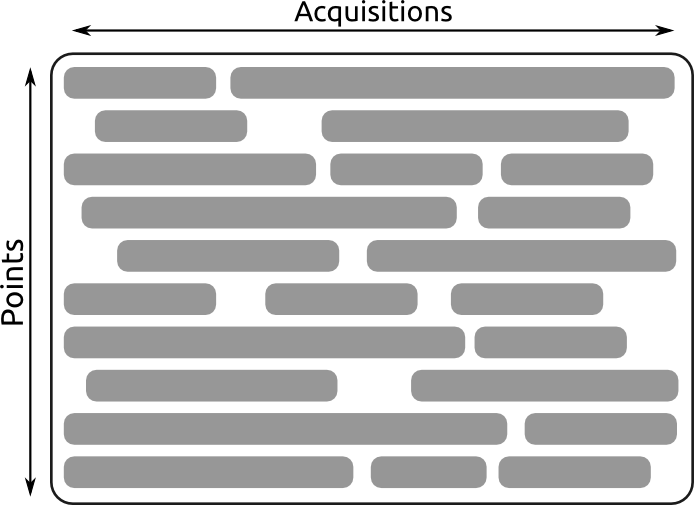
\includegraphics[width=0.6\textwidth]{Chapter4/graphics/visibility_matrix.png}
	\caption{Représentation schématique de la matrice de visibilité}
	\label{fig:ch4_visibility_matrix}
\end{figure}

\subsubsection{Filtrage des points} \label{sec:ch4_filtrage_des_points}
% Plusieurs observations du même point
\paragraph{Observations multiples:\\}
Chaque paire d'image conduisant à l'acquisition d'un nuage de points dans le référentiel du porteur, la détermination de l'ego-motion permet de s'affranchir de ces différences et de ramener toutes les acquisitions dans le même repère. Le suivi de points s'étant par ailleurs effectué dans le temps, on dispose potentiellement pour chaque élément physique observé de nombreuses observations. Le nombre de nuages de points conservés en mémoire tampon (de l'ordre de 200 nuages pour une fenêtre d'intégration de 10 s dans le cas de caméras à 20 images/s) reste le facteur limitant. Il s'agit alors d'obtenir un unique modèle décrivant l'environnement, et d'estimer la meilleure position de chacun de ces éléments.\\

% Optimisation ou filtrage ?
\paragraph{Optimisation ou filtrage:\\}
Deux approches sont alors possibles, comme présenté dans la section \ref{sec:ch4_state_of_art}. Nous pouvons exploiter un algorithme d'optimisation globale appliqué sur une fenêtre glissante (appelé \textit{ajustement de rayons} dans la littérature), ou bien utiliser un estimateur approprié pour obtenir la position de chacun des points. Strasdat \textit{et al.} (\cite{Strasdat2012}) préconisent une approche par filtrage, ce mécanisme assurant pour un coût constant au cours du temps (à nombre de points positionnés égal) la prise en compte de l'ensemble des observations. Une approche par optimisation ne peut prendre en compte l'ensemble des observations et fonctionner en temps constant. Les algorithmes proposés dans la littérature fonctionnent donc souvent sur une fenêtre glissante (seules les observations les plus récentes sont prises en compte, ou bien par sélection d'observations principales (voir par exemple Klein et Murray \cite{Klein2007}, Strasdat \textit{et al}. \cite{Strasdat}, Mei \textit{et al.} \cite{Mei2010})). L'usage d'un estimateur par point apparaissant comme moins coûteux et suffisant en termes de performances, il s'agit de l'approche que nous avons retenue. Il serait cependant possible d'implémenter une solution basée sur un ajustement de rayons pour améliorer la reconstruction de l'environnement à grande échelle, dans un futur développement.

\paragraph{Choix d'un estimateur:\\}
% Filtrage : quel estimateur choisir ? 
Lategahn \textit{et al.} \cite{Lategahn2011} proposent d'utiliser un filtre de Kalman pour estimer individuellement la position des points observés. Les mesures par stéréo-vision sont alors la seule entrée de cet algorithme, qui suppose le point statique et le bruit de position indépendant sur les trois dimensions considérées. Ce filtre revient, dans ce cas, à positionner les points au prorata de la variance de l'estimation et des mesures. Cette approche est relativement coûteuse, eût égard au nombre de points à positionner, et nous avons choisi une estimation plus rapide, que nous supposons suffisante et finalement assez proche en termes de performances. On considère en effet que l'estimation précise du bruit de mesure est de fait un élément difficile des algorithmes de stéréo-vision (fonction du bruit de corrélation entre deux éléments visuels, il n'est pas nécessairement constant et dépendra sans doute de l'environnement visuel du point positionné). Dans ce cadre, nous avons supposé que la plus-value apportée par un filtre de Kalman individuel n'était pas pertinente, et qu'un estimateur plus simple était possible.

\paragraph{Algorithme proposé:\\}
% Notre proposition
L'estimation de la position des points diffère selon deux critères : le points est-il statique ou mobile, est-il encore visible ou non ? Dans le premier cas, on propose d'estimer la position des points par une moyenne pondérée par la distance entre l'élément physique et le plan image lors de l'observation (formulation détaillée dans \ref{eq:ch4_filtrage_pose_points}). Dans ce cas, les points encore visibles sont constamment ré-estimés à chaque nouvelle acquisition, tandis que les points qui ne sont plus visibles sont figés dans un nuage de point statique, que l'on ramène à chaque itération dans le référentiel courant. Si le point est détecté comme un point mobile, selon la méthode précisée dans \ref{sec:ch5_Détection_candidats}, on reporte seulement la position moyennée selon les trois dernières observations. La pondération par la distance lors de l'observation ne rend pas exactement compte de l'ellipse d'incertitude liée au passage dans l'espace en trois dimensions, mais elle nous permet d'en approximer l'amplitude à moindre coût.\\

% Algo
On note dans ce qui suit $X_i^k = (x_i^k, y_i^k, z_i^k)$ le vecteur décrivant la position du point $k$ à l'itération $i$ dans son référentiel courant. On note $X_{j,i}^k$ la position du même point telle qu'observée lors de l'itération $j$ mais ramenée dans le référentiel du porteur lors de l'itération $i$. On note enfin $R_{i,j}$ et $T_{i,j}$ les matrices de transformation permettant de passer du référentiel du porteur lors de l'itération $j$ à celui de l'itération $i$. L'estimation de la position observé depuis l'itération $j$ lors de l'itération $i$ s'écrit alors :

\begin{align}
	X_{j,i}^k	 	&= [R_{i,j} | T_{i,j}] X_j^k \\
	{\hat{X^k}} &= \frac{1}{\nabla} \sum\limits_{l = j}^{i} \frac{X_{l,i}^k}{z_{l}^k}  \label{eq:ch4_filtrage_pose_points}\\
	\nabla 			&= \sum\limits_{l = j}^{i} \frac{1}{z_{l}^k}
\end{align}

La méthode proposée implique de parcourir, pour chaque nouvelle acquisition, l'ensemble des observations passées des points encore visibles pour calculer leur nouvelle position estimée. Ces calculs sont redondants, et le choix d'un estimateur récursif tel qu'une moyenne exponentielle\footnote{Moyenne exponentielle : pour une fenêtre d'intégration de taille $l$, sa valeur est calculée récursivement par: $\hat{X_{l,k}} = \alpha X_k + (1-\alpha) \hat{X_{l,k-1}}$. Le coefficient $\alpha$ est fixe, et vaut: $\alpha = \frac{2}{l + 1}$ } pourrait améliorer le temps de calcul. Le problème de cette méthode serait d'accorder une confiance aux observations fonction du temps, qui n'est pas nécessairement corrélée au réel bruit d'observation (si le porteur s'écarte d'un élément fixe par exemple, le bruit d'observation va croissant). L'utilisation d'un autre estimateur récursif serait peut être possible, bien que la sortie des observations de la mémoire tampon soit à prendre en compte. Ce sujet mériterait certainement des travaux complémentaires.

\section{Implémentation et évaluation} 
\subsection{Ego-Motion}\label{sec:ch4_eval_ego_motion}
Le calcul de l'ego-motion a été implémenté en C++, en utilisant la librairie Eigen\footnote{librairie open-source de calcul matriciel. Pour plus d'informations voir http://eigen.tuxfamily.org} pour le calcul matriciel et l'usage des quaternions. Le temps de calcul est très faible par rapport au reste de notre algorithme, comme présenté dans \ref{sec:ch4_temps_de_calcul}, et approximativement constant.

\subsubsection{Base de données utilisée}
On se base dans la suite sur les données du jeu de données KITTI (\cite{Geiger2012}), qui fournit une vérité terrain à base de centrale inertielle et de GPS. Les acquisitions d'images sont réalisées par des caméras \textit{Point Grey}, à la cadence relativement basse de 10 paires d'images par seconde. La plate-forme d'enregistrement est un véhicule automobile, ce qui explique les vitesses de déplacements relativement élevées pour notre méthode, pouvant monter jusqu'à 10m/s. Les acquisitions représentent un environnement urbain (dans la ville de Karlsruhe) mais aussi des voies rapides.

\subsubsection{Apport de l'UKF}
On évalue tout d'abord l'apport de l'algorithme de filtrage UKF dans la détermination de l'ego-motion, en représentant tout d'abord sur la figure \ref{fig:ch4_egomotion_ukf_raw} les estimations incrémentales du déplacement sur un axe au fil du temps, obtenues de manière brute et après le filtrage proposé comme intégration temporelle.

\begin{figure} 
	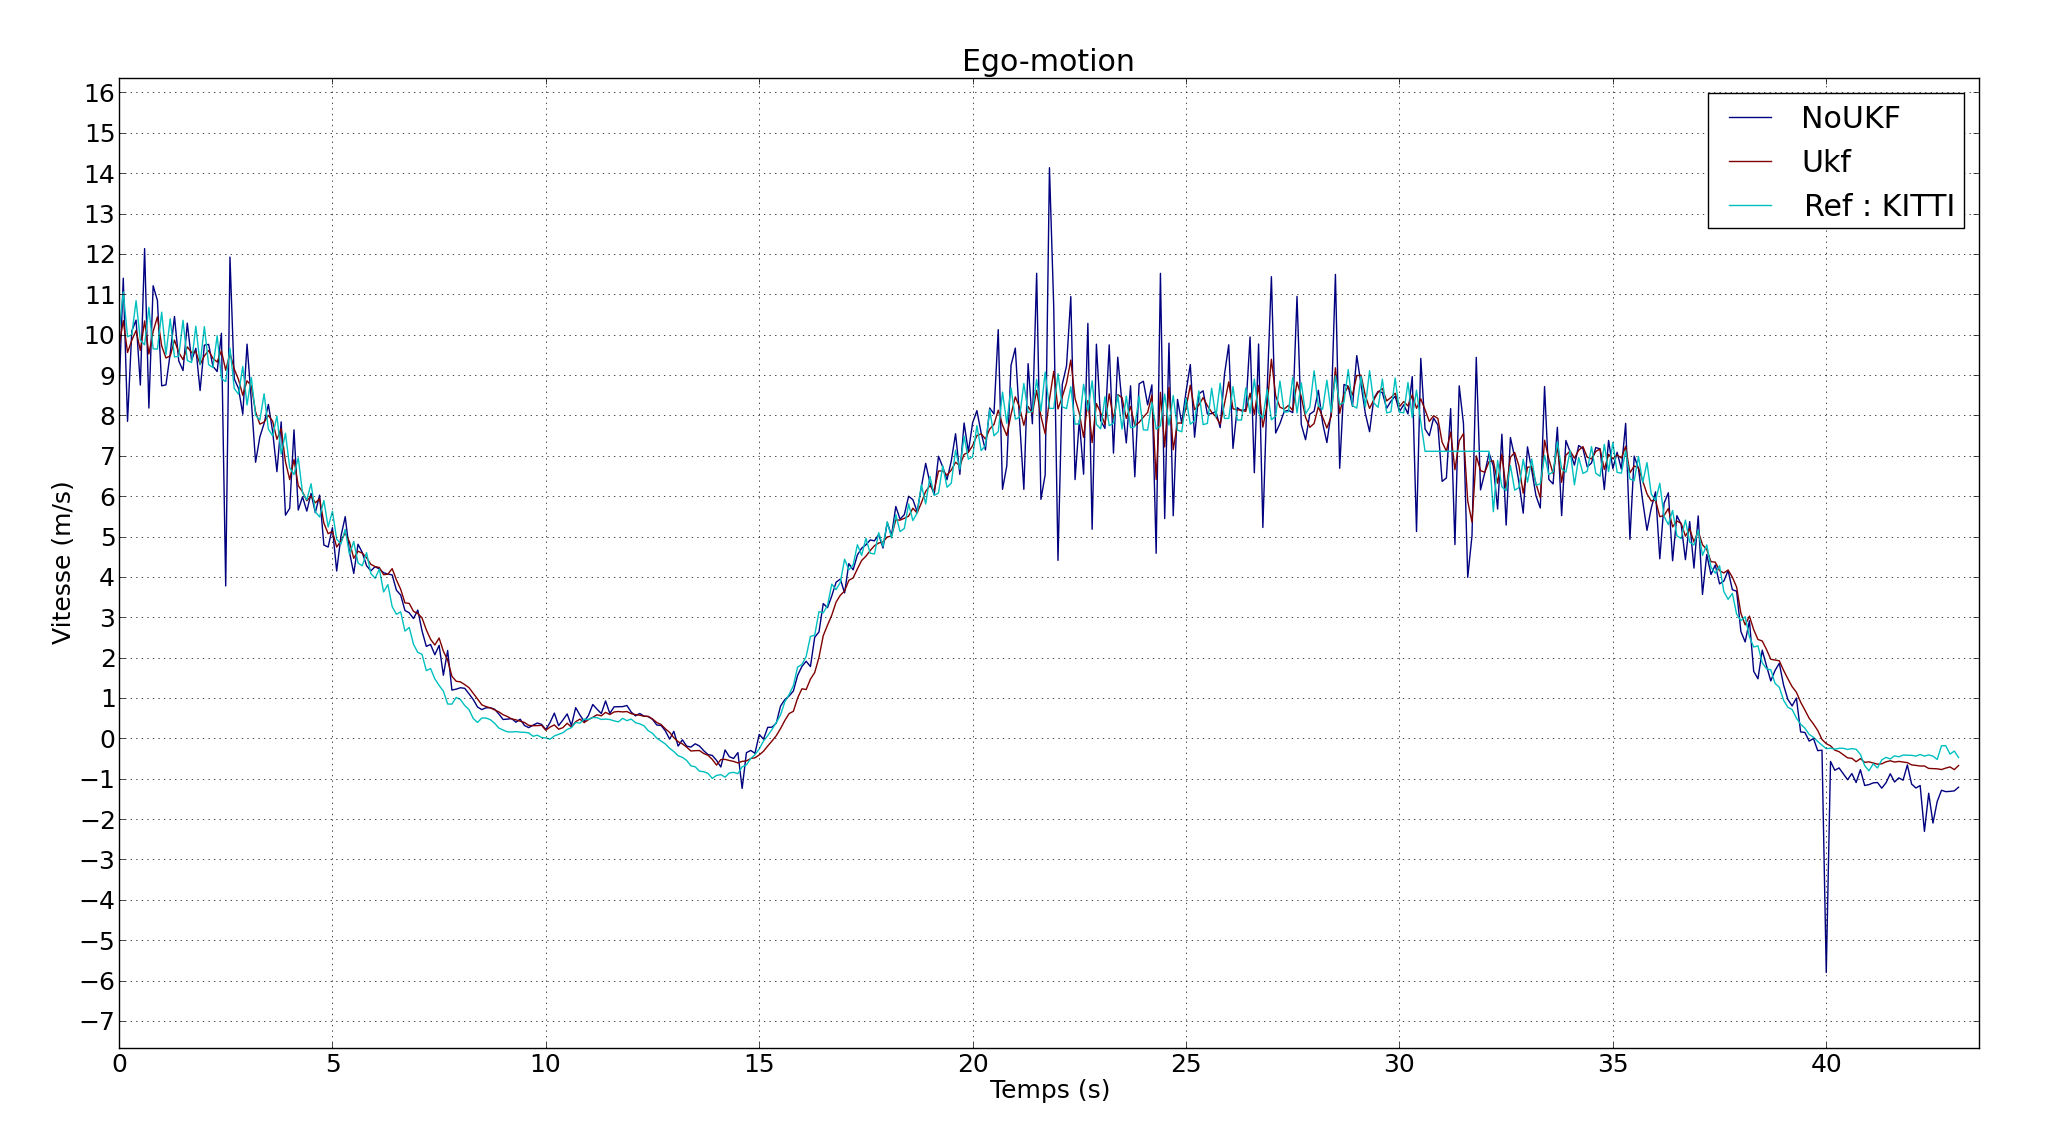
\includegraphics[width=\textwidth]{Chapter4/graphics/ego_motion_UKF_RAW.png}
	\caption{Précision de la détermination de l'ego-motion - comparaison des performances brutes et filtrées. La vitesse est mesurée sur un axe fixe (référentiel initial).}
	\label{fig:ch4_egomotion_ukf_raw}
\end{figure}

On constate aisément que l'estimation du mouvement bénéficie grandement du filtrage proposé en termes de bruit, son coût calculatoire étant, par ailleurs, très faible dans notre implémentation. Les erreurs d'estimation très importantes liées à des mouvements brusques, visibles sur les estimations \og brutes\fg{} sont bien pris en compte par le filtrage, et l'\textit{ego-motion} filtré est qualitativement de qualité très supérieure.\\

\subsubsection{Qualité de l'estimation : comparaison avec l'état de l'art}
On évalue ensuite les performances de notre approche de détermination du mouvement en termes de qualité de positionnement. On se place dans les conditions d'une navigation à l'estime, c'est-à-dire que l'estimation du mouvement propre est la seule information utilisée pour reconstruire les positions successives. \\
Les erreurs de détermination d'angle de rotation conduisent à une erreur de position s'accroissant avec la distance parcourue, phénomène connu sous le nom d'erreur d'Abbe. Les erreurs dans la détermination de la translation sont en général moins influentes, car elles conduisent à une erreur dans le positionnement qui se répartit comme le résultat d'une marche aléatoire, de moyenne nulle dans le cas d'erreurs non-biaisées et qui augmente au fil du temps la largeur de la distribution des positions. \\

\paragraph{Trajectoire obtenue par une marche à l'estime:\\}
La méthode proposée ne comporte pas d'optimisation globale de la trajectoire, qui serait notamment à même d'exploiter une détection des fermetures de boucles. La dérive de la position estimée augmente donc constamment, comme on peut le constater sur la figure \ref{fig:ch4_deadreckoning_overall}. La trajectoire représentée est longue d'environ 1,6 km, très au delà de nos besoins en termes de fenêtre d'intégration (elle représente la trajectoire cumulée observée sur 1900 paires d'images). On utilise un repère orthonormé dont l'origine est le point de départ de la navigation à l'estime.

\begin{figure}[h]
		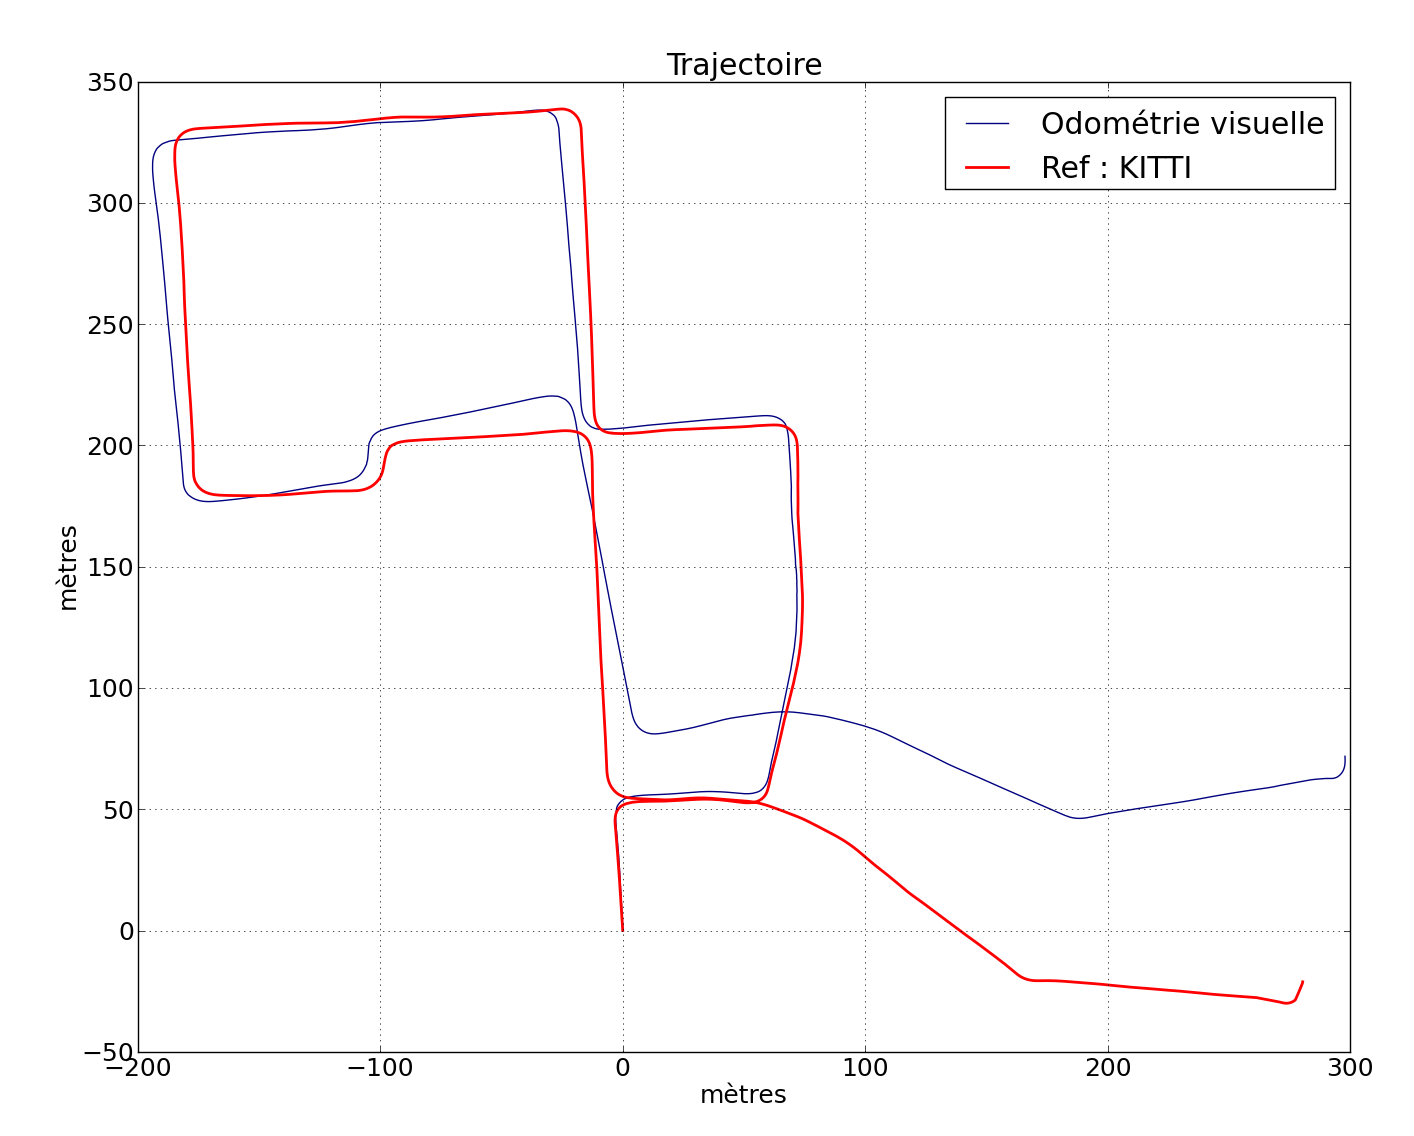
\includegraphics[width=\textwidth]{Chapter4/graphics/dead_reckoning_overall.png}
		\caption{Exemple de navigation à l'estime et de sa dérive cumulée (KITTI - séquence 1). Le point (0,0) constitue le point de départ de la marche à l'estime.}
		\label{fig:ch4_deadreckoning_overall}
\end{figure}

\paragraph{Évaluation quantitative:\\}
L'estimation de la qualité de l'ego-motion demande cependant une représentation plus complète, les résultats obtenus par une comparaison directe des trajectoires de deux méthodes pouvant être trompeurs. L'erreur d'Abbe n'étant pas uniformément répartie en fonction de la distance parcourue, différents points de départ peuvent en effet conduire à des performances \emph{a priori} très différentes. Il est ainsi d'usage de représenter l'erreur en fonction de la distance parcourue, mais en considérant un grand nombre de points de départs possibles sur une séquence donnée, et en moyennant les résultats. On présente donc sur la figure \ref{fig:ch4_error_over_distance} l'erreur de position obtenue par une navigation à l'estime, fonction de la distance parcourue, moyennée sur l'ensemble des tronçons de 400 mètres présents sur la première séquence de la partie \og odométrie\fg{} du jeu de données KITTI (par pas de 10 m, soit environ 150 tronçons). Les interpolations nécessaires sont réalisées de manière linéaire. Le profil observé s'explique par les erreurs de translation et de rotation, qui n'ont pas la même évolution en fonction de la distance parcourue. L'erreur de translation est en effet immédiatement visible, tandis qu'une erreur de rotation n'a initialement qu'un effet limité. L'accumulation des déplacements dans un référentiel erroné en termes de rotation conduit cependant à une erreur fonction croissante de la distance, qui devient donc à terme dominante.

\begin{figure} 
	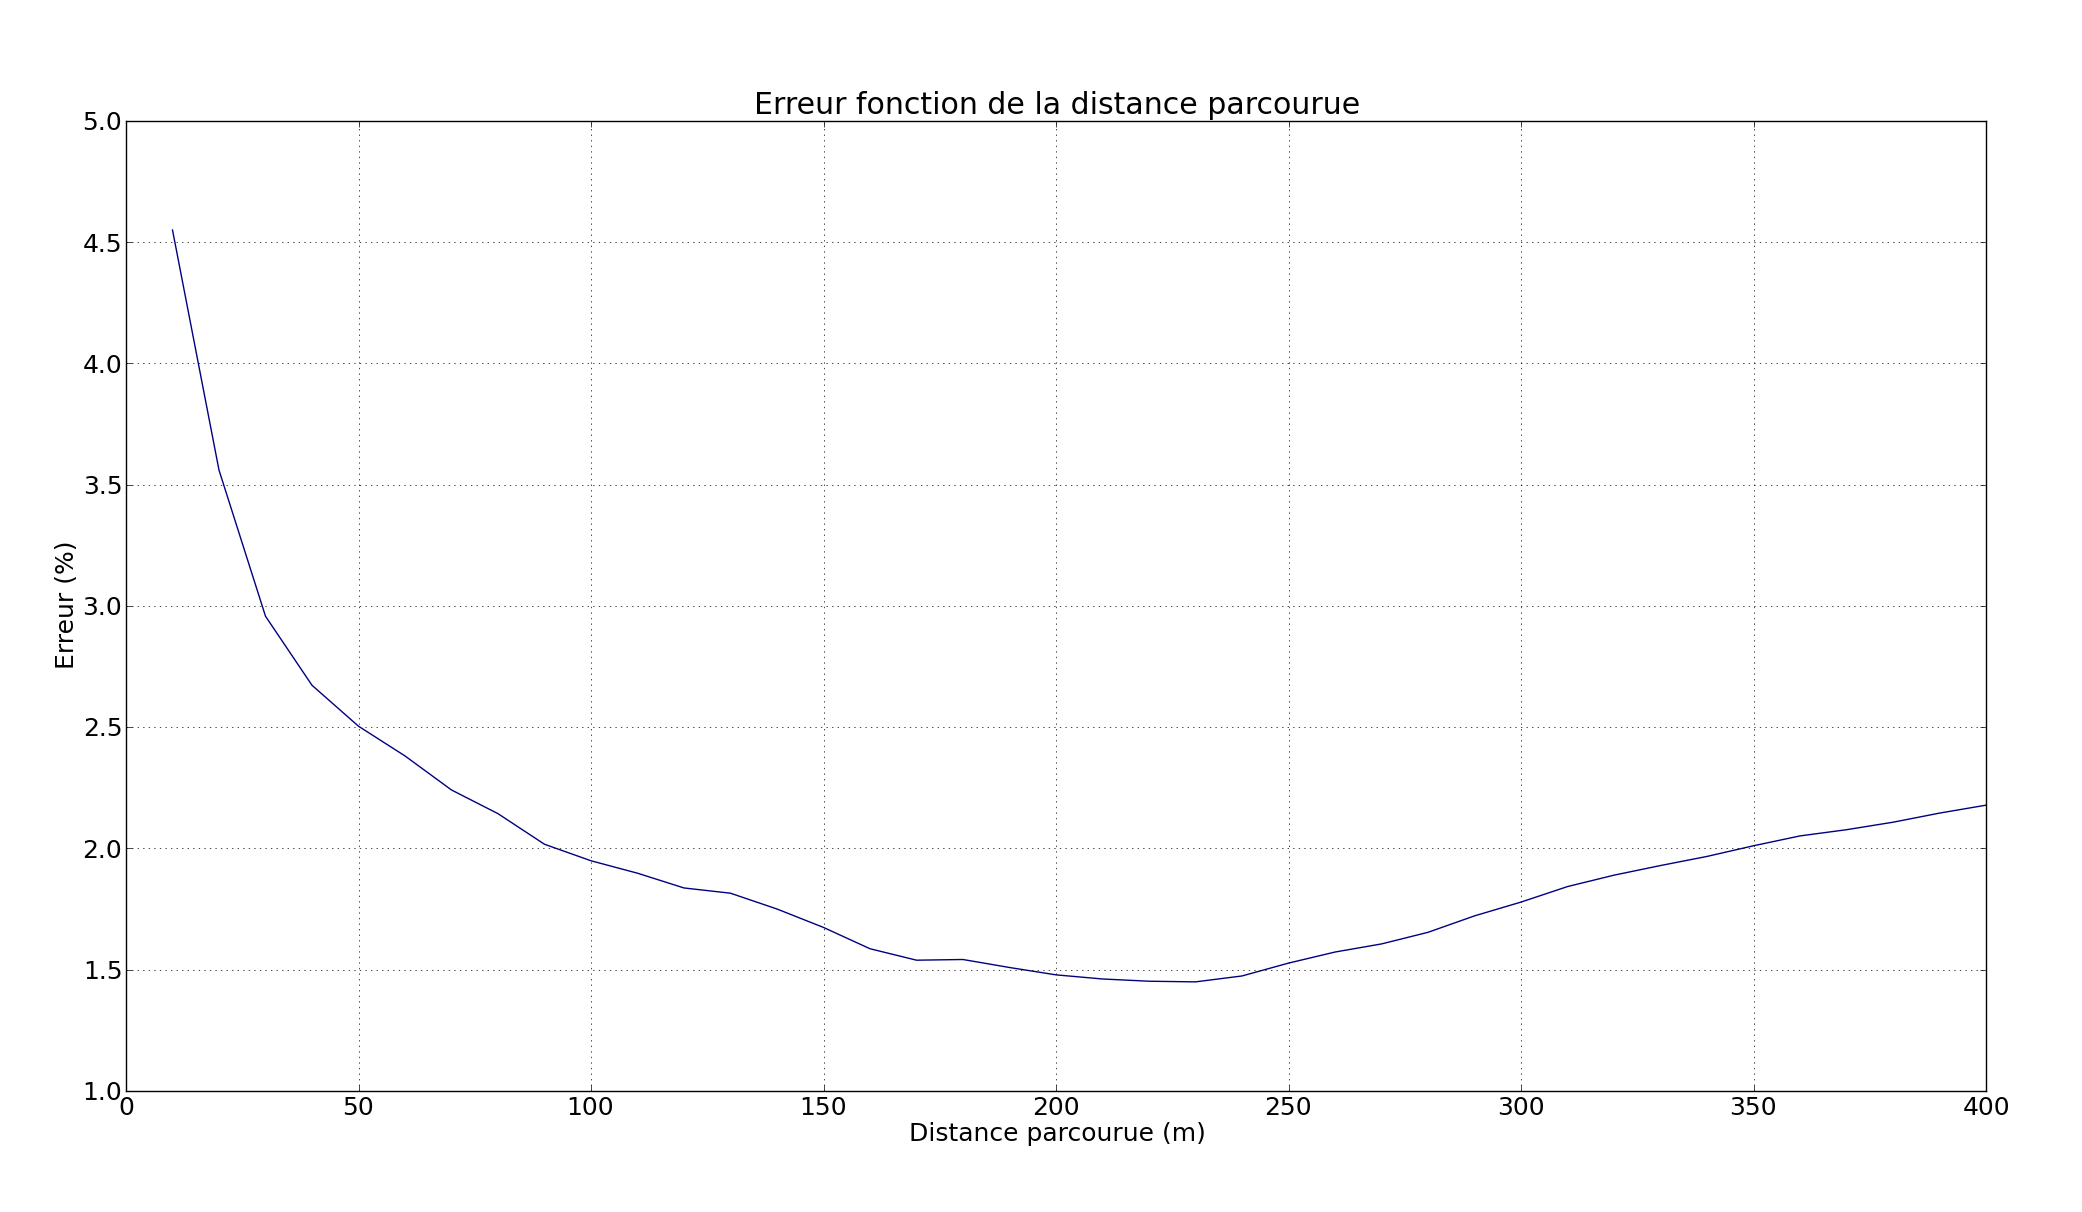
\includegraphics[width=0.8\textwidth]{Chapter4/graphics/error_over_distance_-_sliding_window.png}
	\caption{Erreur de positionnement fonction de la distance parcourue sur l'ensemble des tronçons de 450m possibles (KITTI - séquence 1)}
	\label{fig:ch4_error_over_distance}
\end{figure}

Ces performances sont à comparer à l'état de l'art, et l'on reprend dans le tableau \ref{tab:ch4_résultats_kitti} les résultats présents sur le site de KITTI (\cite{KIT}). Le temps de calcul doit prendre en compte le suivi de points présenté dans le chapitre précédent, et la détermination de l'egomotion que nous présentons ici. Cette dernière est très rapide, comme attendu, puisque qu'elle demande environ 2 ms sur un processeur Intel Core i7 à 2GHz (un seul coeur étant nécessaire). Le suivi de 4000 points sur une plate-forme comparable (CPU donc) demande quant à lui de l'ordre de 45 ms dans les mêmes conditions (suivi de 4000 points).\\

On ne considère cependant ici que la première des séquences proposées par ce jeu de données, contrairement aux autres évaluations présentes dans le tableau, le classement présenté l'étant à titre indicatif. La méthode proposée n'a pas vocation à améliorer l'état de l'art en matière d'odométrie visuelle, ce problème dépassant de loin la problématique de cette thèse qui est axée sur la perception de l'environnement. \\

\begin{table}
	\resizebox{13cm}{!}{
		\centering {
			\begin{tabular}{c | c | c | c | c | c}
				{\bf Classement} & {\bf Méthode} & {\bf Err. Translation} & {\bf Err. Rotation} & {\bf Temps de calcul} & {\bf Plate-forme}\\ \hline
				1 & VoBa 												& 1.77 \% 	& 0.0066 [deg/m] & 0.1 s 	& 1 core @ 2.0 Ghz (C/C++)\\
				2 & VISO2-SAM 									& 1.83 \% 	& 0.0152 [deg/m] & 0.05 s 	& 1 core @ 3.5 Ghz (C/C++)\\
				3 & MFI 												& 1.84 \% 	& 0.0070 [deg/m] & 0.1 s 	& 4 cores @ 3.0 Ghz (C/C++)\\
				4 & eVO 												& 1.93 \% 	& 0.0076 [deg/m] & 0.05 s 	& 2 cores @ 2.0 Ghz (C/C++)\\
				-- & \textbf{Solution proposée} 	& \textbf{1.9 \%} & \textbf{0.015} &  \textbf{0.05s}		&  \textbf{4 cores @ 2.0GHz (C++)}\\
				5 & D6DVO 											& 2.10 \% 	& 0.0083 [deg/m] & 0.03 s 	& 1 core @ 2.5 Ghz (C/C++)\\
				6 & GT\_VO3pt 									& 2.21 \% 	& 0.0117 [deg/m] & 1.26 s 	& 1 core @ 2.5 Ghz (C/C++)\\
				7 & VISO2-S 	& 2.27 \% 				& 0.0152 [deg/m] & 0.05 s 	& 1 core @ 2.5 Ghz (C/C++)\\
				8 & BoofCV-SQ3 	& 2.27 \% 			& 0.0111 [deg/m] & 0.14 s 	& 1 core @ 2.5 Ghz (Java)\\
				9 & TGVO 		& 2.44 \% 					& 0.0105 [deg/m] & 0.06 s 	& 1 core @ 2.5 Ghz (C/C++)\\
				10 & SVO 		& 2.45 \% 					& 0.0109 [deg/m] & 0.05 s 	& 2 cores @ 2.5 Ghz (C/C++)\\
				11 & VO3pt 		& 2.93 \% 				& 0.0116 [deg/m] & 0.56 s 	& 1 core @ 2.0 Ghz (C/C++)\\
				12 & VO3ptLBA 	& 3.17 \% 			& 0.0180 [deg/m] & 0.57 s 	& 1 core @ 2.0 Ghz (C/C++)\\
				13 & KPnP 		& 3.46 \% 				& 0.0144 [deg/m] & 0.2 s 		& 1 core @ 2.5 Ghz (Matlab)\\
				14 & MSD VO 	& 3.50 \% 				& 0.0166 [deg/m] & 0.07 s 	& 1 core @ 2.8 Ghz (C/C++)\\
				15 & MLM-SFM 	& 4.07 \% 				& 0.0104 [deg/m] & 0.03 s 	& 5 cores @ 2.5 Ghz (C/C++)\\
				16 & VOFS 		& 4.21 \% 				& 0.0158 [deg/m] & 0.51 s 	& 1 core @ 2.0 Ghz (C/C++)\\
				17 & VOFSLBA 	& 4.35 \% 				& 0.0189 [deg/m] & 0.52 s 	& 1 core @ 2.0 Ghz (C/C++)\\
				18 & VISO2-M 	& 13.79 \% 				& 0.0372 [deg/m] & 0.1 s 		& 1 core @ 2.5 Ghz (C/C++)\\
			\end{tabular}
		}
	}	
	\caption{Résultats de différentes méthodes sur le jeu de données KITTI. Notre méthode n'est évaluée que sur la première séquence, contrairement aux autres résultats (11 séquences)}
	\label{tab:ch4_résultats_kitti}
\end{table}

\subsection{Reconstruction 3D}
La reconstruction de l'environnement a été également implémentée en C++, en utilisant là encore la librairie Eigen pour les calculs matriciels, et la structure \emph{PointCloud} de la librairie PCL (\emph{Point Cloud Library}, \cite{Rusu2011}) pour le stockage des nuages de points. Cette étape est également très rapide, étant essentiellement limitée dans le nombre de points traités par leur stockage en mémoire courante. \\
Une évaluation quantitative de la reconstruction est difficile, faute de vérité terrain aisément comparable, nous présentons donc une comparaison avec l'environnement obtenu par un capteur de type \emph{Velodyne}, le HDL64. La qualité de la reconstruction en trois dimensions est difficile à appréhender sur une projection, d'autant plus que la répartition des points diffère entre les deux procédés, mais on peut notamment remarquer que les plus gros obstacles (voitures, éléments de voirie) sont bien visibles sur le squelette reconstitué. Les nuages de points obtenus par ces deux procédés sont présentés sur la figure \ref{fig:ch4_comparaison_velodyne}. Le nuage de point \emph{Velodyne} correspond à une unique acquisition tandis que le nuage de points que nous présentons correspond à une intégration temporelle, l'objectif n'est donc pas d'évaluer les mérites respectifs de ces approches mais bien plus d'exploiter une vérité terrain obtenue par le télémètre laser.\\

\begin{figure}[h]
	\begin{center}
		\begin{subfigure}{1.0\textwidth}
			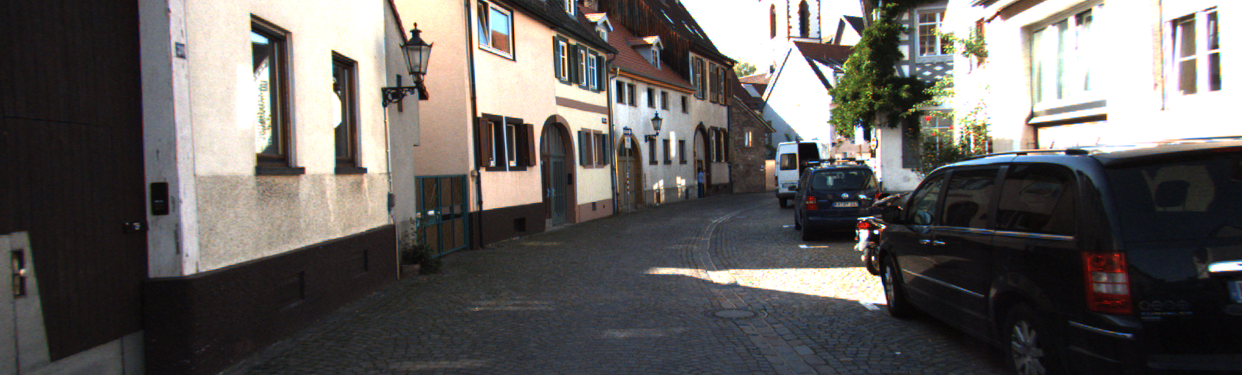
\includegraphics[width=\textwidth]{Chapter4/graphics/KITTI_pict.png} 
			\caption{Vue de la caméra}
		\end{subfigure}	
		\newline
		\begin{subfigure}[t]{0.48\textwidth}
			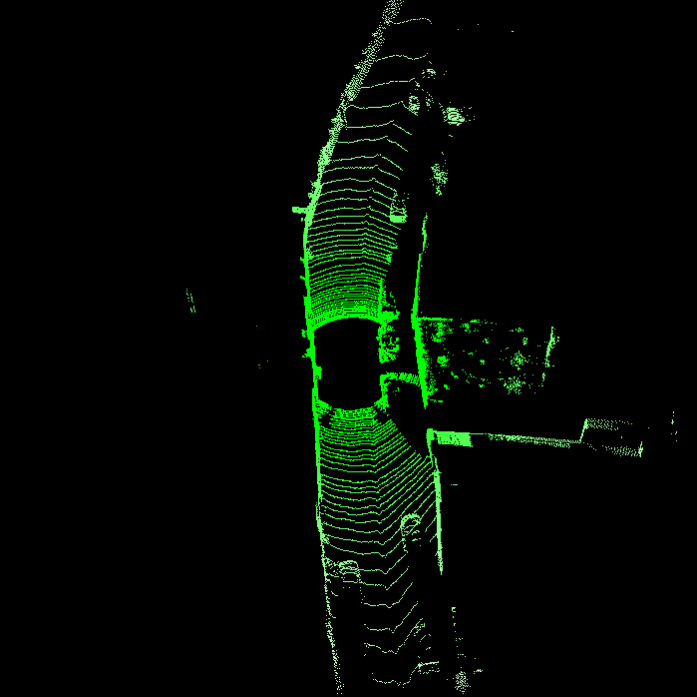
\includegraphics[width=\textwidth]{Chapter4/graphics/KITTI_Velodyne.png} 
			\caption{Nuage de points instantané du capteur HDL64. Vue aérienne}
		\end{subfigure}	
		~
		\begin{subfigure}[t]{0.48\textwidth}
			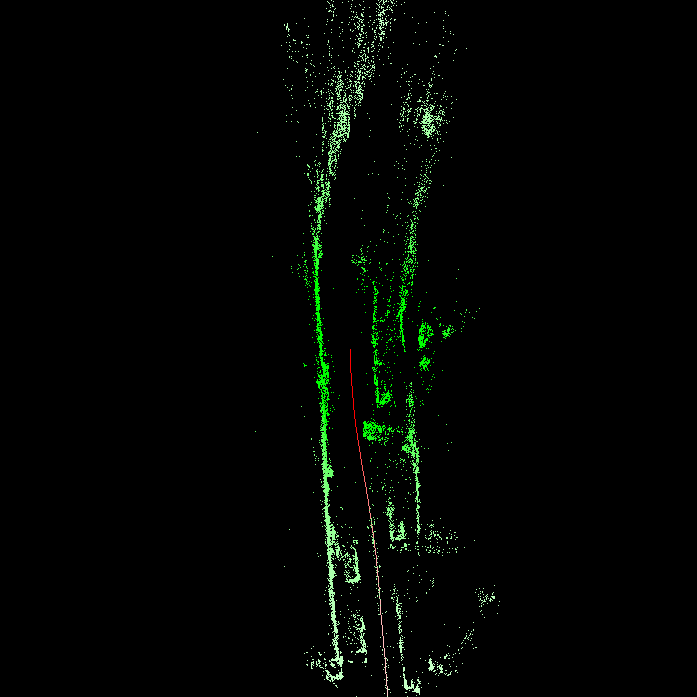
\includegraphics[width=\textwidth]{Chapter4/graphics/KITTI_SLAM_1.png} 
			\caption{Nuage de points obtenu par notre méthode, et trajectoire estimée du véhicule. Vue aérienne}
		\end{subfigure}	
		
		\caption{Comparaison des nuages de points obtenus par un télémètre laser Velodyne HDL64 (b) et par notre proposition (c)(Données issues de KITTI). Le temps de calcul décrit la période minimale entre deux acquisitions, et comprend l'ensemble des étapes  de l'algorithme (suivi de points dans l'image, estimation de l'ego-motion et reconstruction 3D dans notre cas).}
		\label{fig:ch4_comparaison_velodyne}
	\end{center}
\end{figure}

\subsection{Temps de calcul} \label{sec:ch4_temps_de_calcul}
La problématique du calcul temps réel est respectée sans trop de difficultés par cette étape de notre algorithme. Cette étape rajoute une latence qui reporte les étapes suivantes, mais ne restreint pas la cadence de traitement, dans la mesure où le suivi de points dans l'image reste le facteur limitant (cf. section \ref{sec:ch6_temps_reel}). Notre implémentation est réalisée en C++, avec l'aide de la librairie Eigen pour le calcul matriciel, et exploite plusieurs processus parallèles. La plate-forme de test utilise un processeur de type Intel Core i7 à 2GHz, les quatres unités d'exécution présentes étant utilisées.\\
On représente à la fois sur la figure \ref{fig:ch4_temps_de_calcul} l'évolution du temps de calcul et celle du nombre de points présents dans l'environnement modélisé. Le jeu de données utilisé est celui de KITTI (\cite{Geiger2012}), acquis depuis une plate forme automobile dans un environnement urbain. On maintient un ensemble de 4000 points suivis sur les paires d'images stéréoscopiques exploitées, 100 acquisitions étant ensuite prises en compte dans la construction du squelette représentatif de l'environnement. Du fait de la cadence d'acquisition de 10 images par seconde sur ce jeu de données, les 10 dernières secondes d'observation sont donc prises en compte dans l'environnement représenté.\\

\begin{figure}[h] 
	\centering
	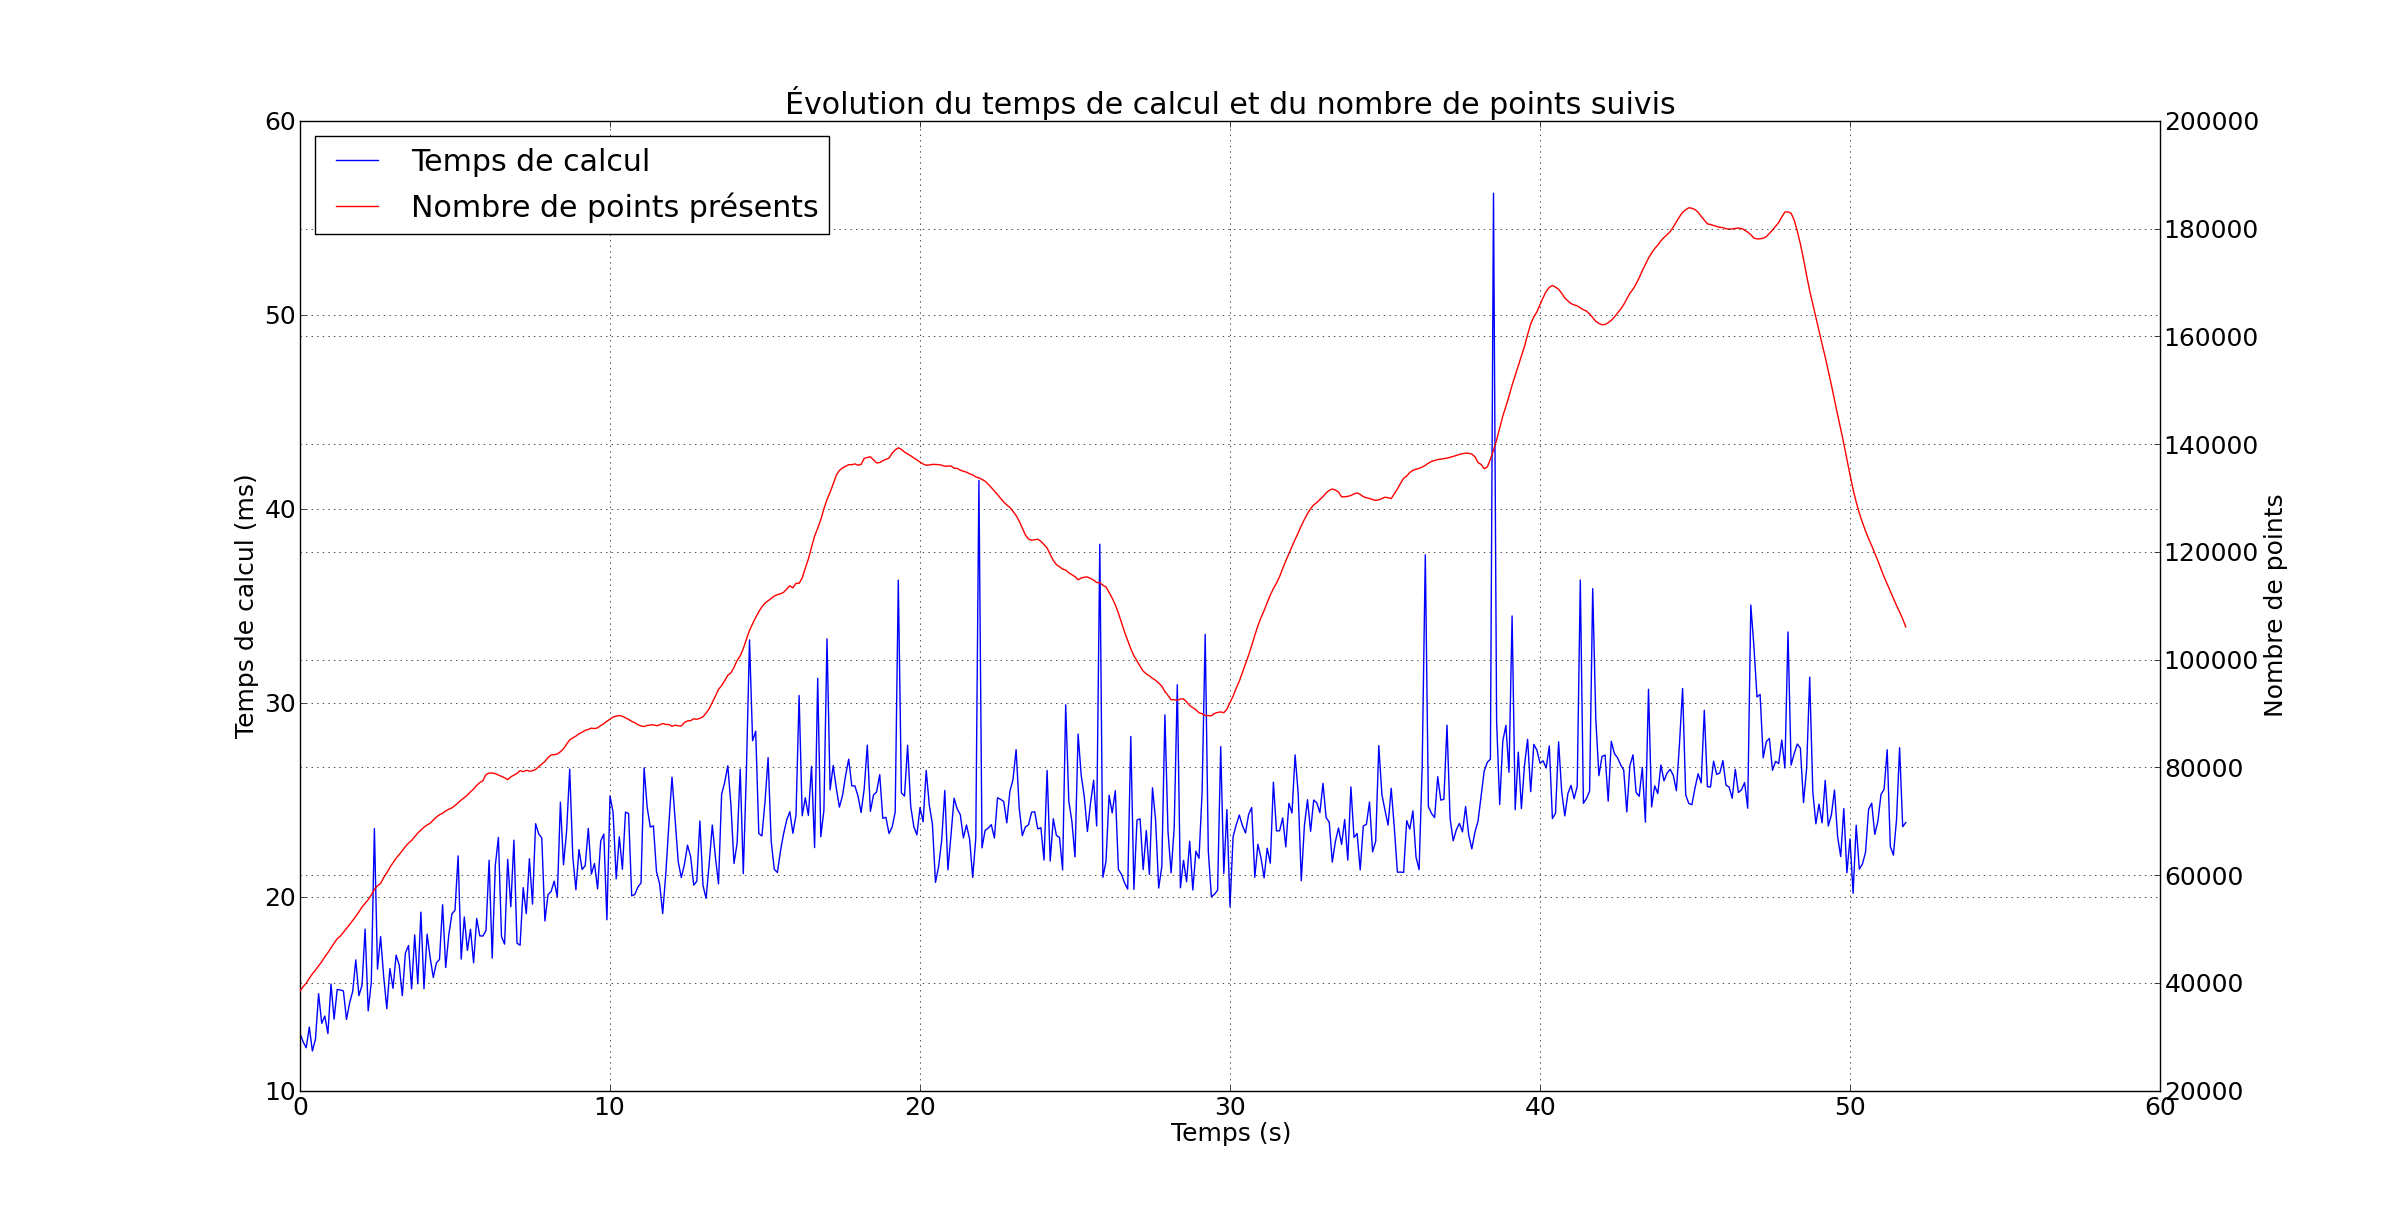
\includegraphics[width=0.98\textwidth]{Chapter4/graphics/computing_time.png}
	\caption{Exemple d'évolution du temps de calcul global de cette étape (ego-motion et reconstruction de l'environnement). Les fluctuations s'expliquent en partie par une variation du nombre de points observés ou en mémoire.}
	\label{fig:ch4_temps_de_calcul}
\end{figure}

On peut remarquer sur la figure \ref{fig:ch4_temps_de_calcul} que le temps de calcul augmente en fonction du nombre de points présents, comme attendu. Tous les points présents n'ont cependant pas le même coût de propagation, la position des points encore visibles étant réévaluée à chaque nouvelle observation, tandis que les points qui ne sont plus visibles sont représentés par leur dernière position estimée, et simplement ramenés dans le référentiel courant (section \ref{sec:ch4_filtrage_des_points}). Les fluctuations constatées dans le temps de calcul sont alors liées à la sortie des points observés du champ de vision. Certains déplacements peuvent ainsi influer rapidement sur le nombre de points sortant du champ de vision (virages brusques par exemple), ce qui explique, au moins partiellement, les variations du temps de calcul observées. Le nombre de points présents dans le squelette est borné par le nombre de nuages conservés en mémoire tampon, de même que le temps de calcul. On constate aisément que celui-ci est compatible avec une cadence d'acquisition élevée (cette étape pouvant traiter plus de 30 acquisitions par seconde en moyenne).\\

\subsection{Quelle fenêtre d'intégration ?}
Nous souhaitons ici améliorer notre perception de l'environnement en cumulant les observations selon une fenêtre temporelle d'intégration, dont l'étendue est de l'ordre de 100 paires d'images. Cette fenêtre d'intégration est limitée par deux facteurs : une contrainte d'implémentation (augmenter sa taille a un impact - assez faible relativement à l'ensemble du procédé - sur le temps de calcul, et demande plus de place en mémoire), et une contrainte environnementale. Il est ainsi inutile de cumuler les observations sur une échelle de temps très supérieure au temps de présence des éléments suivis dans le champ de vision. Celui-ci varie en fonction du déplacement du véhicule et du déplacement des objets de la scène, son estimation est délicate, mais on constate empiriquement qu'une fenêtre temporelle de 10 secondes est bien supérieure au temps de présence effectif de la majorité des éléments du champ de vision.\\

Une remarque peut être faite en termes d'ordre de grandeur, pour valider notre accumulation temporelle d'informations. On peut en effet comparer l'erreur introduite dans la reconstruction de l'environnement par la marche à l'estime le long de la fenêtre d'intégration, par rapport aux erreurs typiques liées à une observation de stéréo-vision. En supposant une vitesse d'environ 10 m/s et une cadence d'acquisition de 10 im/s, pour rester dans les conditions de l'évaluation ci-dessus, l'erreur attendue par la navigation à l'estime pendant l'accumulation est de l'ordre de 2m\footnote{Il s'agit d'un cas extrême, et l'erreur est dans ce cas concentrée sur les points les plus lointains.}. Une erreur de 0.5 pixels dans la détermination de la position d'un élément de la scène sur le plan image, pour un point dont la disparité initiale est de 3 pixels et avec les conditions des mesures précédentes, conduit à une erreur dans son positionnement dans l'espace de 15m. Il s'agit bien sûr d'un  calcul très grossier, mais il illustre l'intérêt du filtrage dans le temps des observations, en dépit de l'erreur réalisée sur la compensation du mouvement.

\section{Conclusion}
On a présenté dans ce chapitre une solution originale de détermination de l'\textit{ego-motion} à partir de points suivis sur une paire stéréo-vision, à un coût calculatoire très faible. Cette solution est suffisamment précise pour l'intégration temporelle que nous effectuons, qui nous permet de reconstruire la position des points suivis au fil du temps et de réduire un bruit d'observation très important dans un dispositif de stéréo-vision. \\
Du fait de la séparation entre ces deux tâches, nous montrons également que le nombre de points traités  en temps réel peut être très important, de l'ordre de plusieurs dizaines de milliers de points sur une plate-forme mobile grand public. Un récapitulatif de ces différentes étapes est visible sur la figure \ref{fig:ch4_vue_ensemble_algo}.\\

On dispose à ce moment d'un modèle de la scène environnant le porteur, grâce à des points positionnés dans l'espace. Ce modèle ne vaut que pour les points statiques, les points détectés comme mobiles nécessitant alors un traitement plus approfondi.

\begin{figure}[h] 
	\centering
	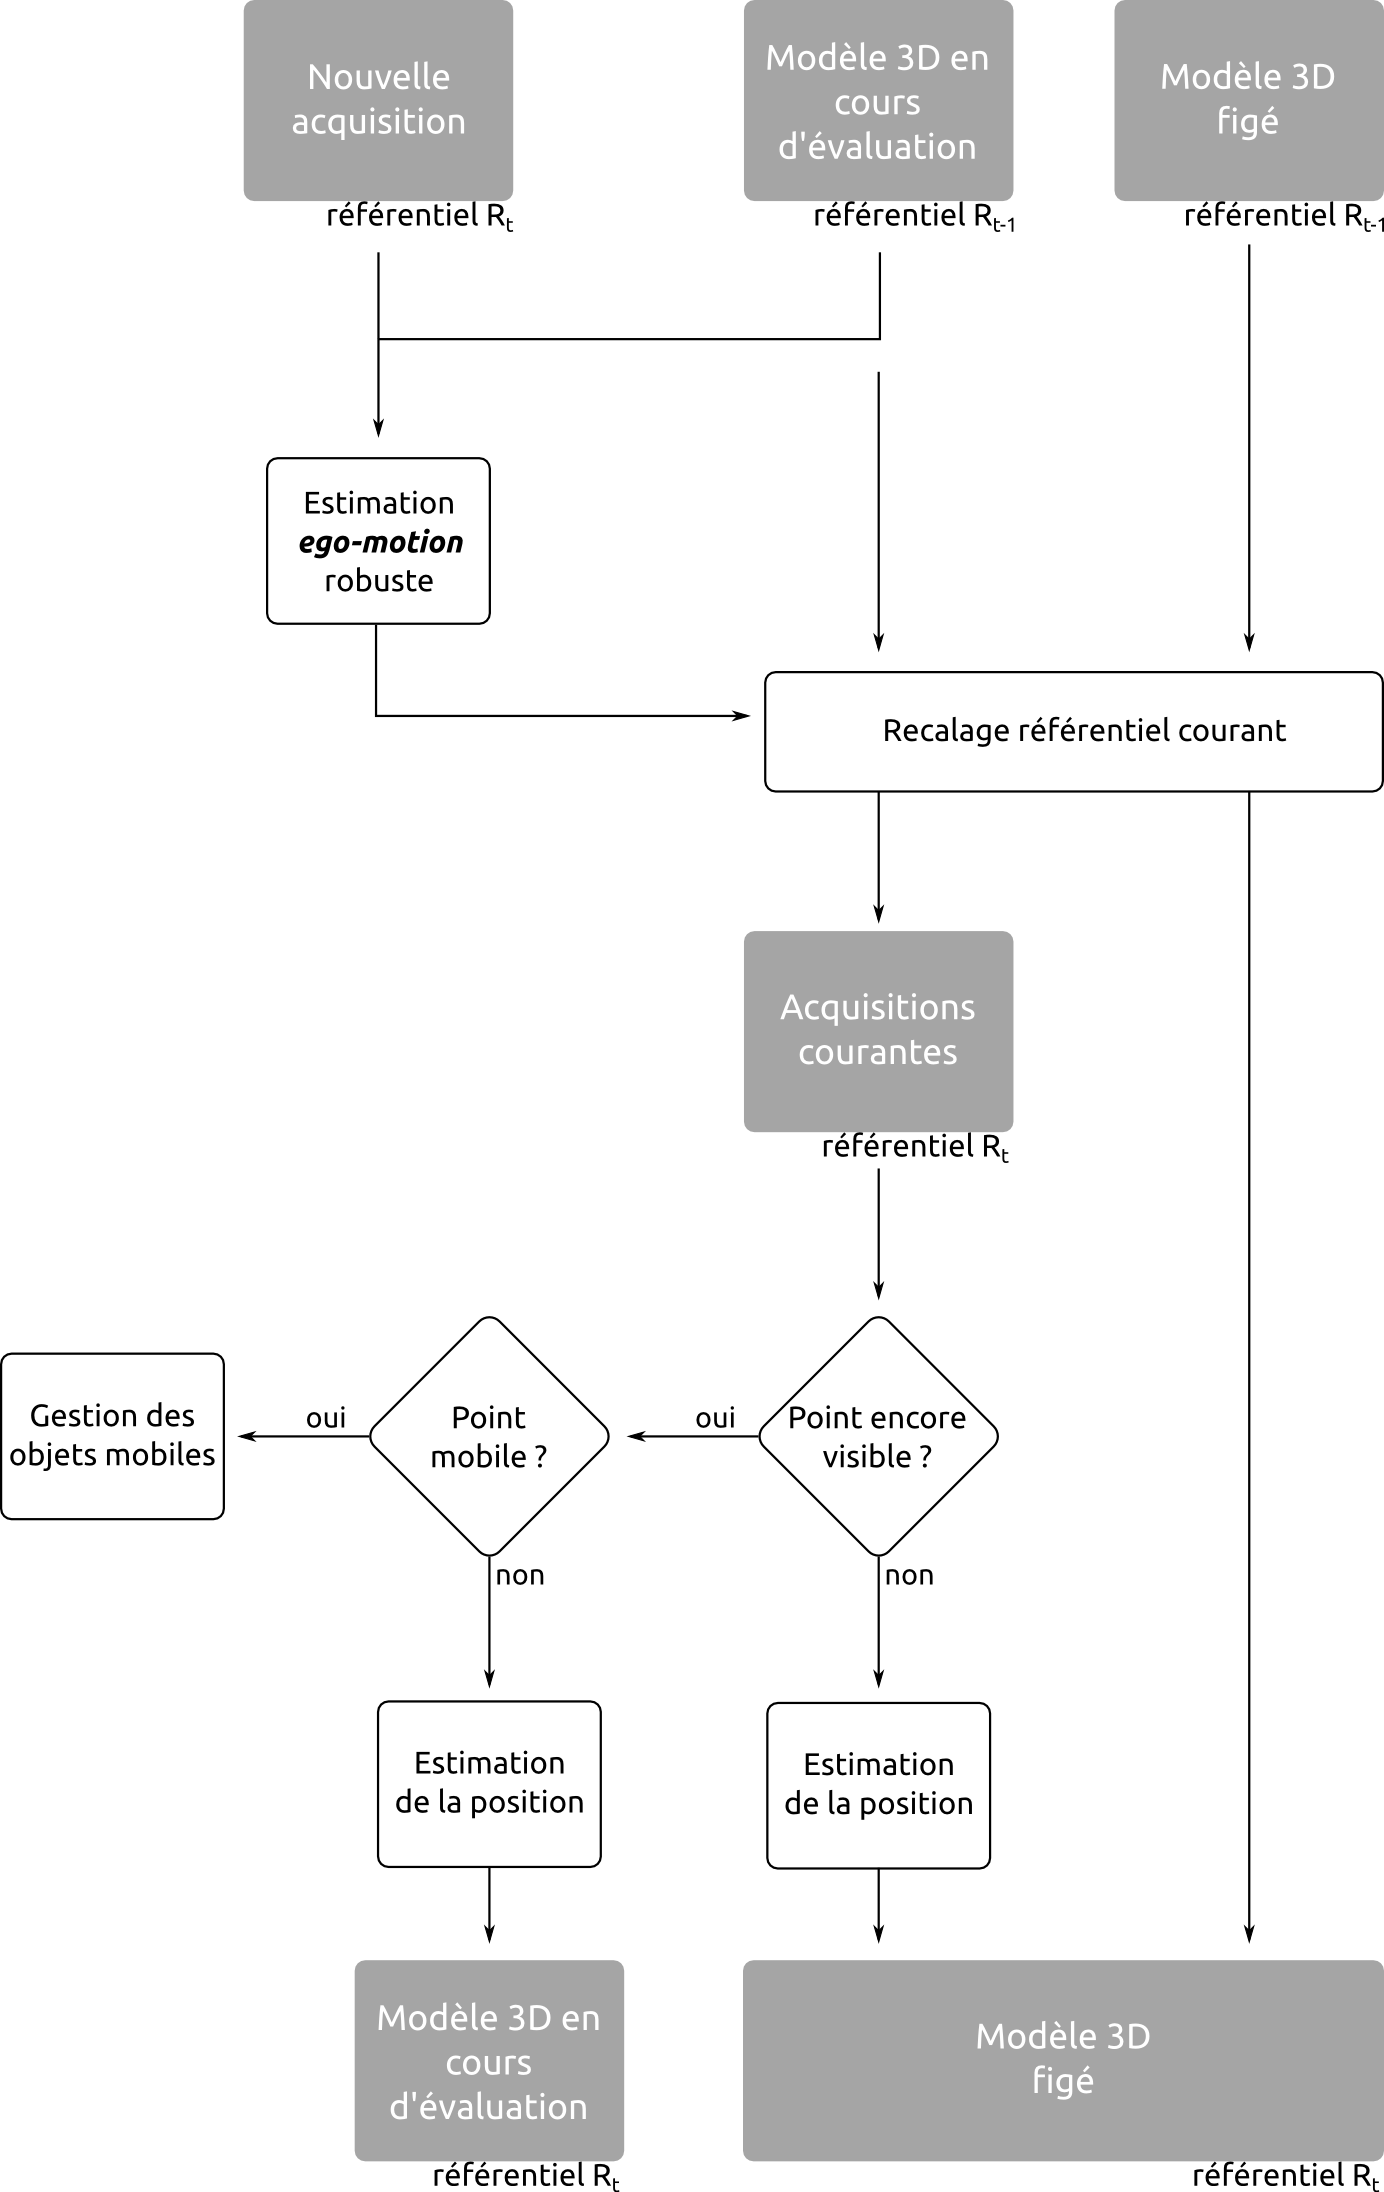
\includegraphics[width=0.98\textwidth]{Chapter4/graphics/detailled_scheme.png}
	\caption{Vue d'ensemble de l'algorithme proposé.}
	\label{fig:ch4_vue_ensemble_algo}
\end{figure}
